\documentclass[11pt,a4paper]{article}

\usepackage[margin=2.5cm]{geometry}
\usepackage{amsmath,amssymb}
\usepackage{graphicx}
\usepackage{booktabs}
\usepackage[numbers,sort&compress]{natbib}
\usepackage{hyperref}
\usepackage{xcolor}

\graphicspath{{../../../Toy_Characterisation/Verify_new_results/outputs/segment_analysis/}
              {../../../Toy_Characterisation/Verify_new_results/outputs/segment_analysis/paper/}
              {../../../Toy_Characterisation/Verify_new_results/outputs/segment_analysis/segment_analysis/}}

\newcommand{\nt}{n_\text{tracks}}
\newcommand{\sss}{\sigma_s}
\newcommand{\srr}{\sigma_r}
\newcommand{\eps}{\varepsilon}

\title{Segment- and Track-level Validation of the \texttt{lhcb\_velo\_toy} Model:\\
       A Hopfield-Hamiltonian Reconstruction Stress Test up to $10^3$ Tracks per Event}

\author{G.~Scriven\\[2pt]\textit{Nikhef, Amsterdam}}

\date{\today}

\begin{document}

\maketitle

\begin{abstract}
We report a comprehensive validation of the \texttt{lhcb\_velo\_toy} simulation and
reconstruction stack --- a five-plane VeLo-like toy detector coupled to a
Hopfield-style Hamiltonian segment solver --- against an earlier reference
implementation, and extend the characterisation regime to $\nt = 1000$
tracks per event. Using an analytically motivated angular acceptance
$\eps(\sss,\srr)$ we verify that (i) the segment-matching efficiency
stays pinned at $100\%$ across the full range of physical noise and track
multiplicity, (ii) the classical Hamiltonian solver delivers $100\%$
segment efficiency up to $\nt = 1000$ with false activation rate rising
from $0$ at low multiplicity to $\approx 20\%$ at $\nt=1000$, (iii) the
matrix spectrum remains strictly positive ($\lambda_\mathrm{min} \geq 0.88$, condition
number $\kappa \leq 9$), and (iv) the dominant failure mode at high
$\nt$ is \emph{post-processing} --- the default connected-components
tracker merges false-segment bridges into mega-clusters and collapses
reconstruction efficiency from $99\%$ to $43\%$ between $\nt = 300$ and
$\nt = 1000$, whereas a layer-exclusive tracker restores efficiency to
$\gtrsim 99.9\%$ at the cost of a $23.6\%$ ghost rate. The validated
operating point for the Hamiltonian segment solver is
$(\gamma,\delta,\eps,\tau) = (3,\,1,\,2\,\mathrm{mrad},\,0.35)$.
\end{abstract}

%--------------------------------------------------------------------
\section{Introduction}\label{sec:intro}

The \texttt{lhcb\_velo\_toy} package is a lightweight VeLo-like detector
simulator and reconstruction framework used to prototype Hopfield-style
\cite{Hopfield:1982,Denby:1988,Peterson:1989,Stimpfl-Abele:1991} and
quantum \cite{Funcke:2023:qtracking,Nilles:2023:qtracking} track-finding
algorithms on realistic multiplicities. This report addresses four
specific questions regarding its correctness and operating envelope:
\begin{enumerate}
  \item Does the analytic angular threshold $\eps(\sss,\srr)$ faithfully
        match the true-segment angle distribution under realistic
        multiple-scattering and hit-resolution noise?
  \item Does the package reproduce the segment-level acceptance curves of
        the older reference notebook \texttt{track\_density\_test\_local.ipynb}
        when parameters are matched?
  \item How does the classical Hopfield Hamiltonian solver scale up to
        $\nt = 1000$, in terms of (a) segment efficiency, (b) false-rate
        survival, (c) spectral conditioning, and (d) track-level
        reconstruction metrics?
  \item Where does the stack fail first, and is that failure in the
        solver, the acceptance model, or the post-processing tracker?
\end{enumerate}

The analysis is carried out in a single master notebook
\texttt{segment\_level\_analysis.ipynb} with 17 sections, whose structure
is mirrored in this report. All figures referenced below are cached
artefacts in \texttt{outputs/segment\_analysis/} and were not
regenerated for this write-up.

%--------------------------------------------------------------------
\section{Model and methodology}\label{sec:method}

\subsection{Detector and event generator}
The detector consists of five parallel plane modules spaced by
$\Delta z = 33$~mm, centred on $z \in \{33,66,99,132,165\}$~mm, each of
active area $80 \times 80\ \mathrm{mm}^2$ (half-width $40$~mm) except
for the \S\ref{sec:fixed-eps} reference-reproduction experiment, which
uses $160 \times 160\ \mathrm{mm}^2$ for parameter matching to the
earlier study. Primary vertices are drawn from a Gaussian with
$\sigma_{xyz} = (0,0,1)$~mm in the default sweeps and $(1,1,1)$~mm in
the reference-reproduction experiment.
Tracks are generated by
\texttt{lhcb\_velo\_toy.generation.StateEventGenerator} with uniform
$\phi\in[-\phi_\mathrm{max},\phi_\mathrm{max}]$ and identical
$\theta$-cone. Hit positions are perturbed by a Gaussian measurement
error $\srr$; the propagation direction is perturbed at each module by
a multiple-scattering kick $\sss$.

\subsection{Angular acceptance $\eps$}
A segment \emph{pair} sharing a common middle hit is accepted if the
opening angle between the two segments is below a threshold $\eps$
computed as
\begin{equation}
  \eps(\sss,\srr) \;=\; \sqrt{\,2\,\theta_s^2 \;+\; 12\,\theta_r^2 \;+\; 2\,\theta_\mathrm{min}^2\,},
  \label{eq:eps}
\end{equation}
with $\theta_s = s\,\sss$, $\theta_r = \arctan(s\,\srr/\Delta z)$,
$s = 3$, and $\theta_\mathrm{min} = 1.5\times 10^{-5}$~rad.
The factor $12$ on the hit-resolution term propagates the kink due to
independent resolution errors on both segments through the triplet.
The $\theta_\mathrm{min}^2$ floor guarantees a non-zero threshold even
in the zero-noise limit.

\subsection{Segment-pair definitions}
Two definitions are used in parallel:
\begin{enumerate}
  \item \emph{Shared-middle-hit (triplet)}:
        all ordered triples of hits $(h_{p},h_{m},h_{n})$ on
        consecutive modules. A pair is \emph{true} iff both
        component segments belong to the same truth track. Combinatorics
        $\mathcal{O}(T^3)$.
  \item \emph{Pairwise (truth segments only)}:
        one segment per truth-track consecutive-hit pair, all
        $\binom{N_\mathrm{seg}}{2}$ pairs enumerated; true iff both
        segments are from the same truth track. Combinatorics
        $\mathcal{O}(T^2)$.
\end{enumerate}
The two methods share the true-pair population exactly but differ by
orders of magnitude in the false-pair pool and thus in the predicted
false-acceptance rate. All sweeps are evaluated in both methods and
cross-checked against pure-Python reference kernels before using the
Numba-JIT \cite{Lam:2015:numba} accelerated versions for large
multiplicities.

\subsection{Hopfield Hamiltonian and solver}
The segment Hamiltonian $H(\gamma,\delta)$ is constructed by
\texttt{SimpleHamiltonianFast} with penalty $\gamma = 3$ and bias
$\delta = 1$. Its off-diagonal entries reward angle-consistent
same-module-chain segment pairs and penalise hit-sharing conflicts;
the diagonal is $(\delta+\gamma)$ so that for an isolated segment the
Hopfield fixed point is $s^\ast = \delta/(\delta+\gamma) = 0.25$. The
full system $H s = b$ is solved by direct sparse Cholesky
(SciPy); a threshold $\tau = 0.35$ separates active segments ($s_i
\geq \tau$) from inactive ones. For an isolated five-hit truth chain
the outermost-segment fixed point is the geometric invariant
$s^\ast_\mathrm{outer} = 0.3636\ldots$ which is used as a solver
health-check throughout.

\subsection{Trackers}
Two post-processors are compared: \texttt{get\_tracks} assembles
connected components from the set of active segments, and
\texttt{get\_tracks\_layered} is a module-exclusive greedy variant
seeded at the first module that enforces angular consistency between
consecutive segments.

\subsection{Validation}
Reconstructed tracks are matched against the truth with
\texttt{EventValidator.match\_tracks} using LHCb-standard cuts
(purity $\geq 0.70$, \texttt{min\_rec\_hits} $= 3$)
\cite{LHCbVELO:TDR}.

\subsection{Implementation checks}
All Numba kernels are byte-validated against pure-Python references
before deployment; the custom vectorised Hamiltonian builder used in
\S\ref{sec:solver} is \emph{exactly} (matrix- and vector-equal) the
same assembly as \texttt{SimpleHamiltonianFast.construct\_hamiltonian}
\cite{Lehoucq:1998:arpack}.

%--------------------------------------------------------------------
\section{Segment-level results}\label{sec:segment}

\subsection{Baseline (\S3, \S4)}
Figure~\ref{fig:baseline} shows the true- and false-pair angle
distributions for a single event of $20$ tracks at $\sss=0.1$~mrad,
$\srr=0$. The true peak is confined well below the analytic $\eps$;
the false distribution has bulk density at tens of mrad. The
scattering-sweep histograms confirm that $\eps$ tracks the mean of
the true-angle distribution across $\sss \in [0.05,1.0]$~mrad and
keeps the true-pair acceptance above $80\%$ while leaving the false
tail unaffected.

\begin{figure}[t]
  \centering
  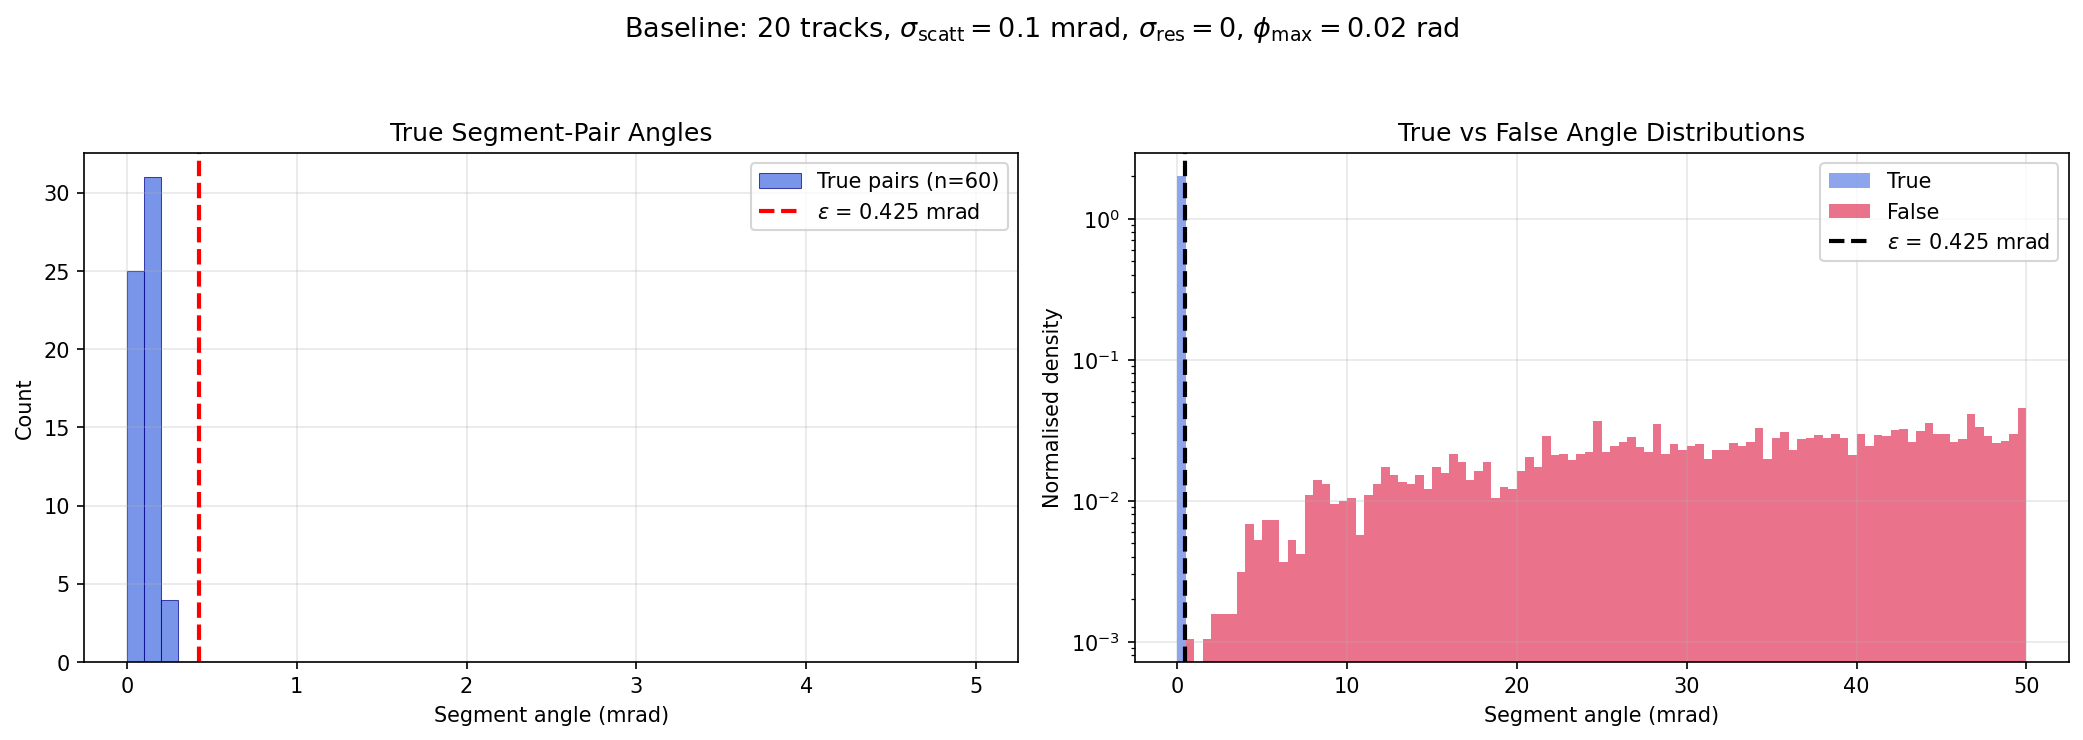
\includegraphics[width=0.7\linewidth]{baseline_angle_distributions.png}
  \caption{Pair-angle distributions for a baseline event (20 tracks,
  $\sss=0.1$~mrad, $\srr=0$). Dashed line: analytic $\eps$ from
  Eq.~\eqref{eq:eps}. Source: segment\_level\_analysis.ipynb~\S3.}
  \label{fig:baseline}
\end{figure}

\subsection{Scattering and resolution sweeps (\S5, \S6)}\label{sec:sweeps}
For $\nt\in\{10,20,50,100\}$, $\sss\in\{0.05,\dots,1.0\}$~mrad and
$\srr\in\{0,5,\dots,50\}$~$\mu$m, the segment efficiency
(true-pair acceptance) is pinned at $100\%$ across both angle cones
$\phi_\mathrm{max}\in\{0.02,0.2\}$
(Fig.~\ref{fig:sweeps}). The false-rate climbs monotonically with
noise, as expected because $\eps$ widens. The resolution term
dominates above $\srr \gtrsim 20\ \mu\mathrm{m}$ as anticipated
from the $12\theta_r^2$ coefficient in Eq.~\eqref{eq:eps}.

\begin{figure}[t]
  \centering
  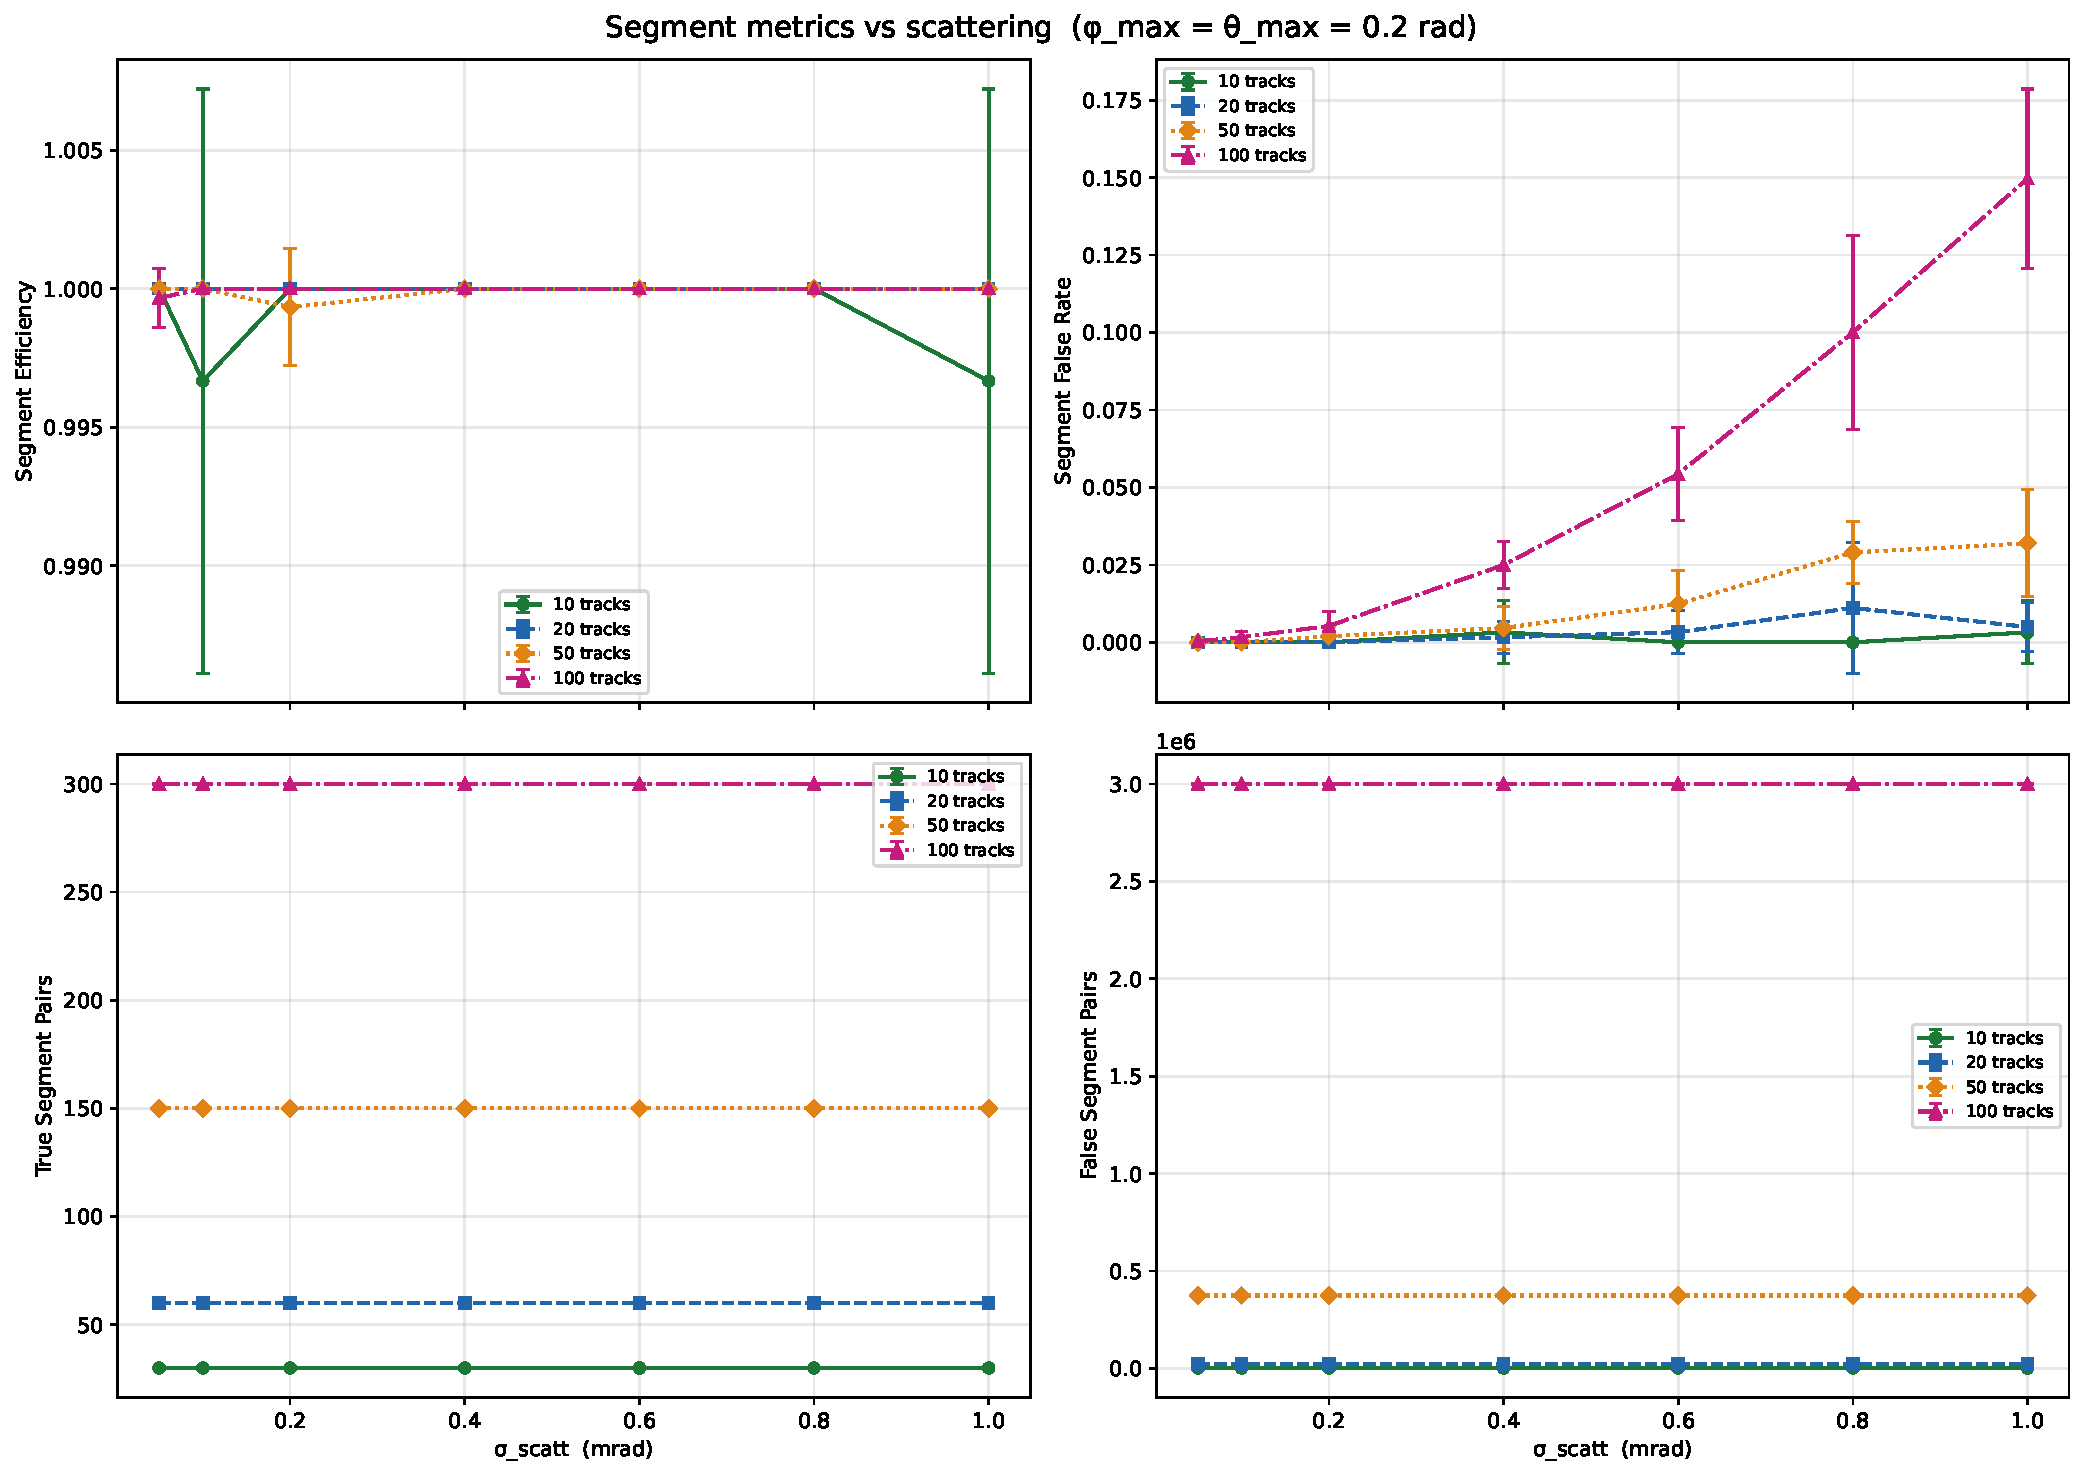
\includegraphics[width=0.48\linewidth]{scattering_sweep_phi0.2.pdf}\hfill
  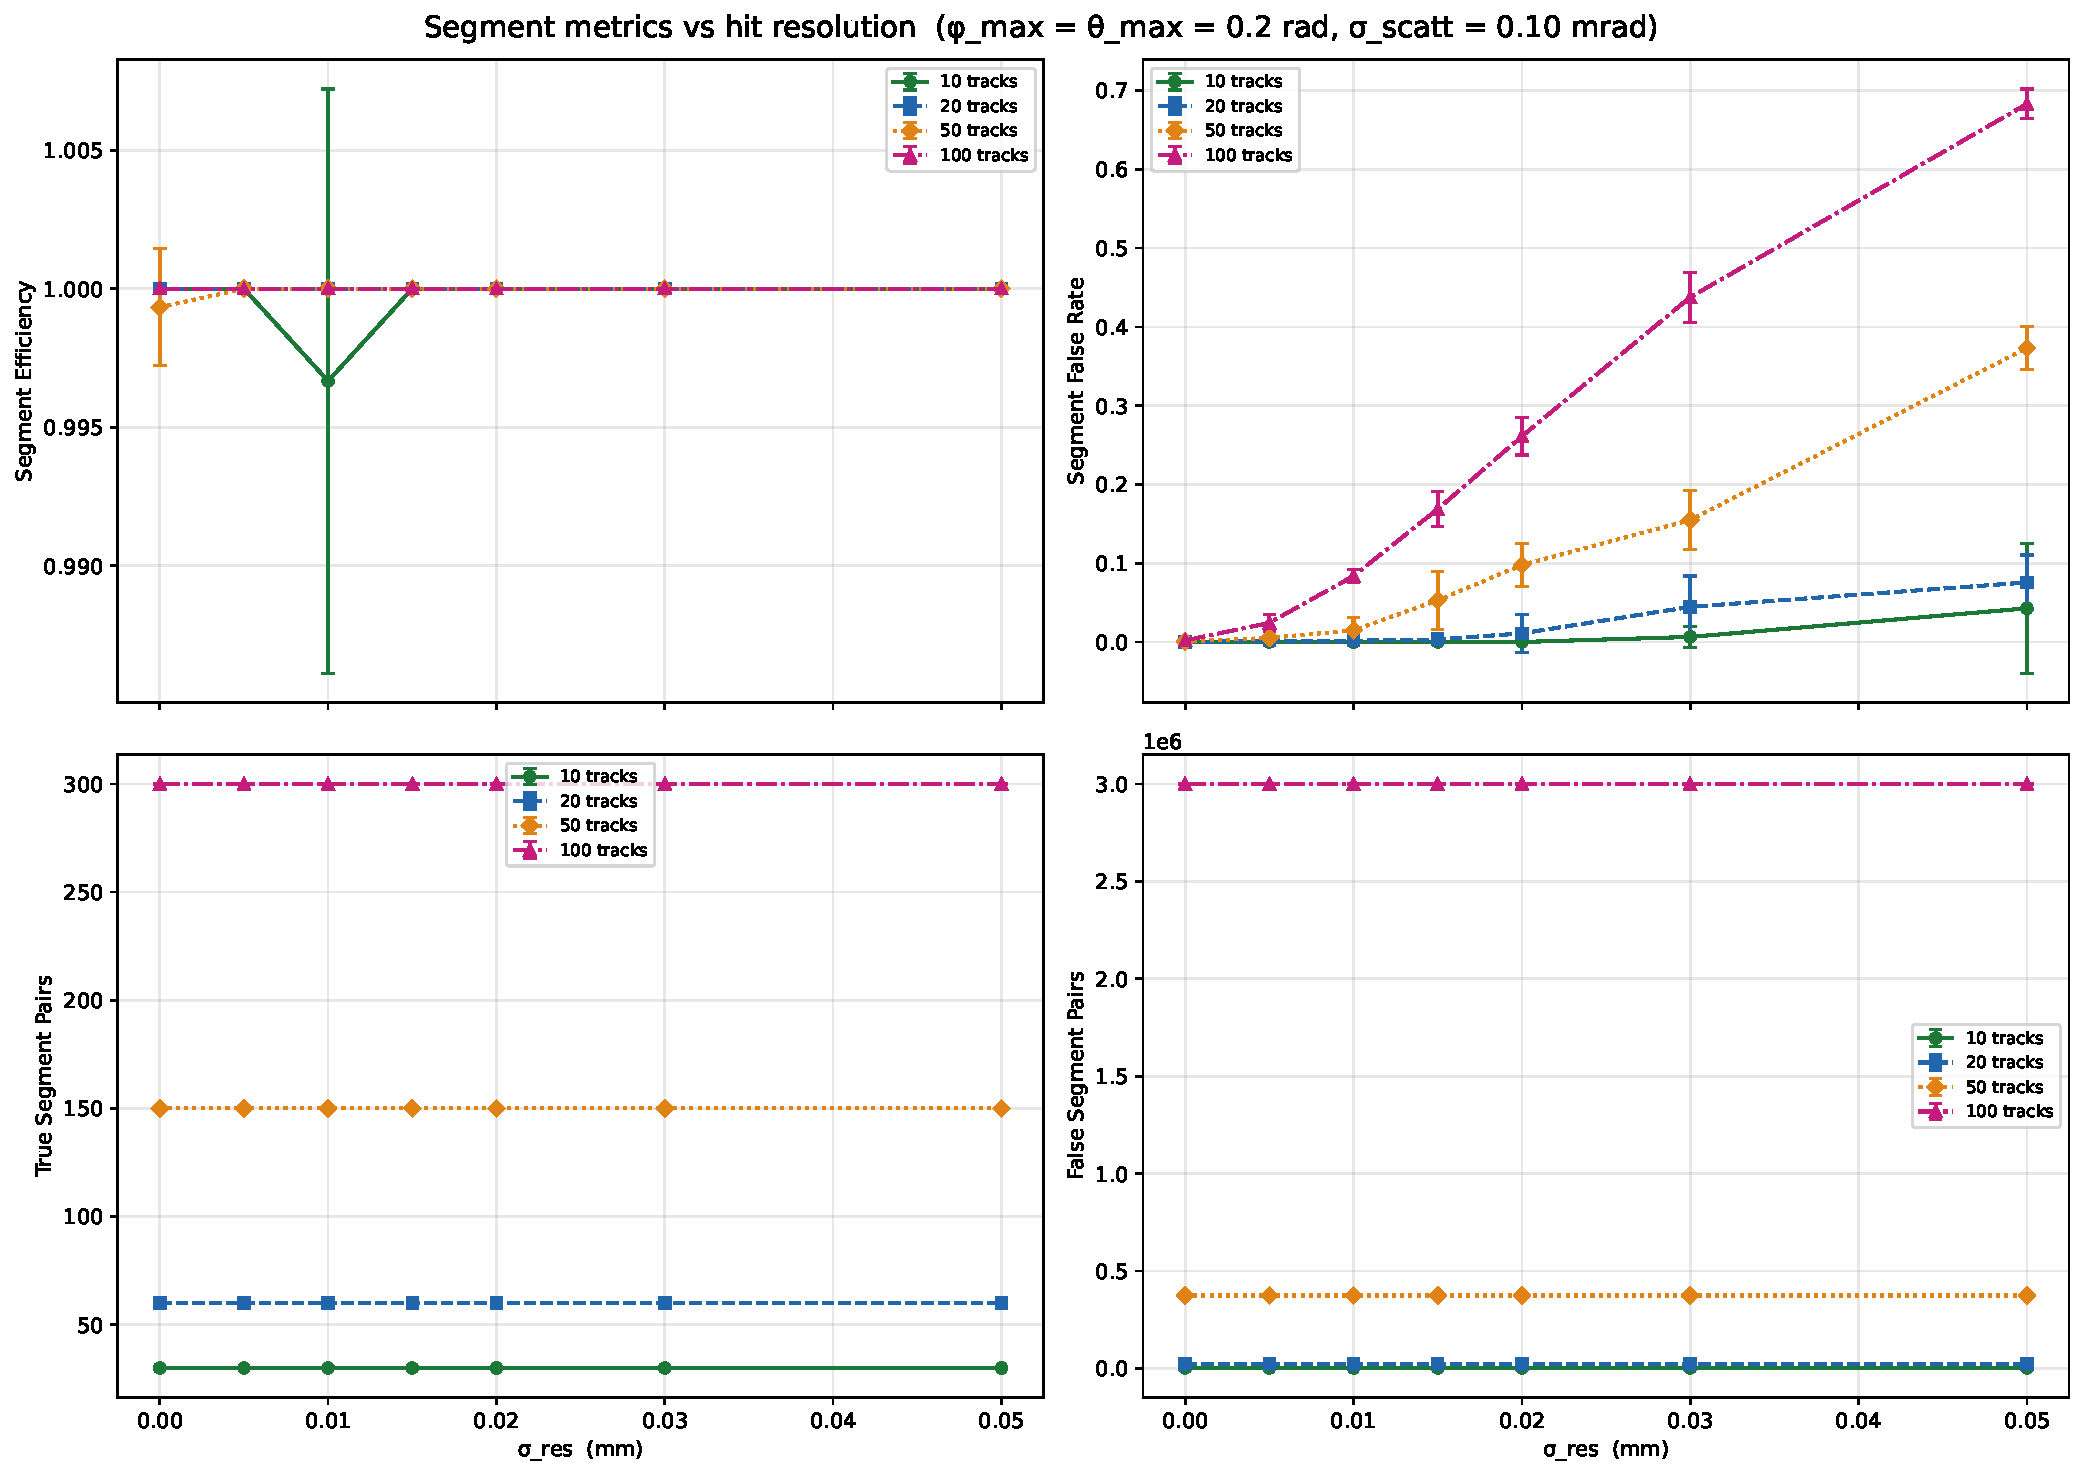
\includegraphics[width=0.48\linewidth]{resolution_sweep_phi0.2.pdf}
  \caption{Scattering (left) and resolution (right) sweeps at
  $\phi_\mathrm{max}=0.2$. Segment efficiency stays at $100\%$;
  false rate grows monotonically with noise.}
  \label{fig:sweeps}
\end{figure}

\subsection{Density scan and ROC (\S7, \S8)}
Figure~\ref{fig:density} plots segment efficiency, false rate, and
raw true/false pair counts versus $\nt$ at fixed noise. True pairs
scale as $\nt$; false pairs as $\nt^3$ (triplet method), confirmed by
the reference $n^3$ line in panel~(d). The ROC acceptance curves
(not shown) place the analytic $\eps$ operating point on the knee
between $>98\%$ true-acceptance and $\lesssim 1\%$ false-acceptance
for all tested $\sss \leq 0.4$~mrad.

\begin{figure}[t]
  \centering
  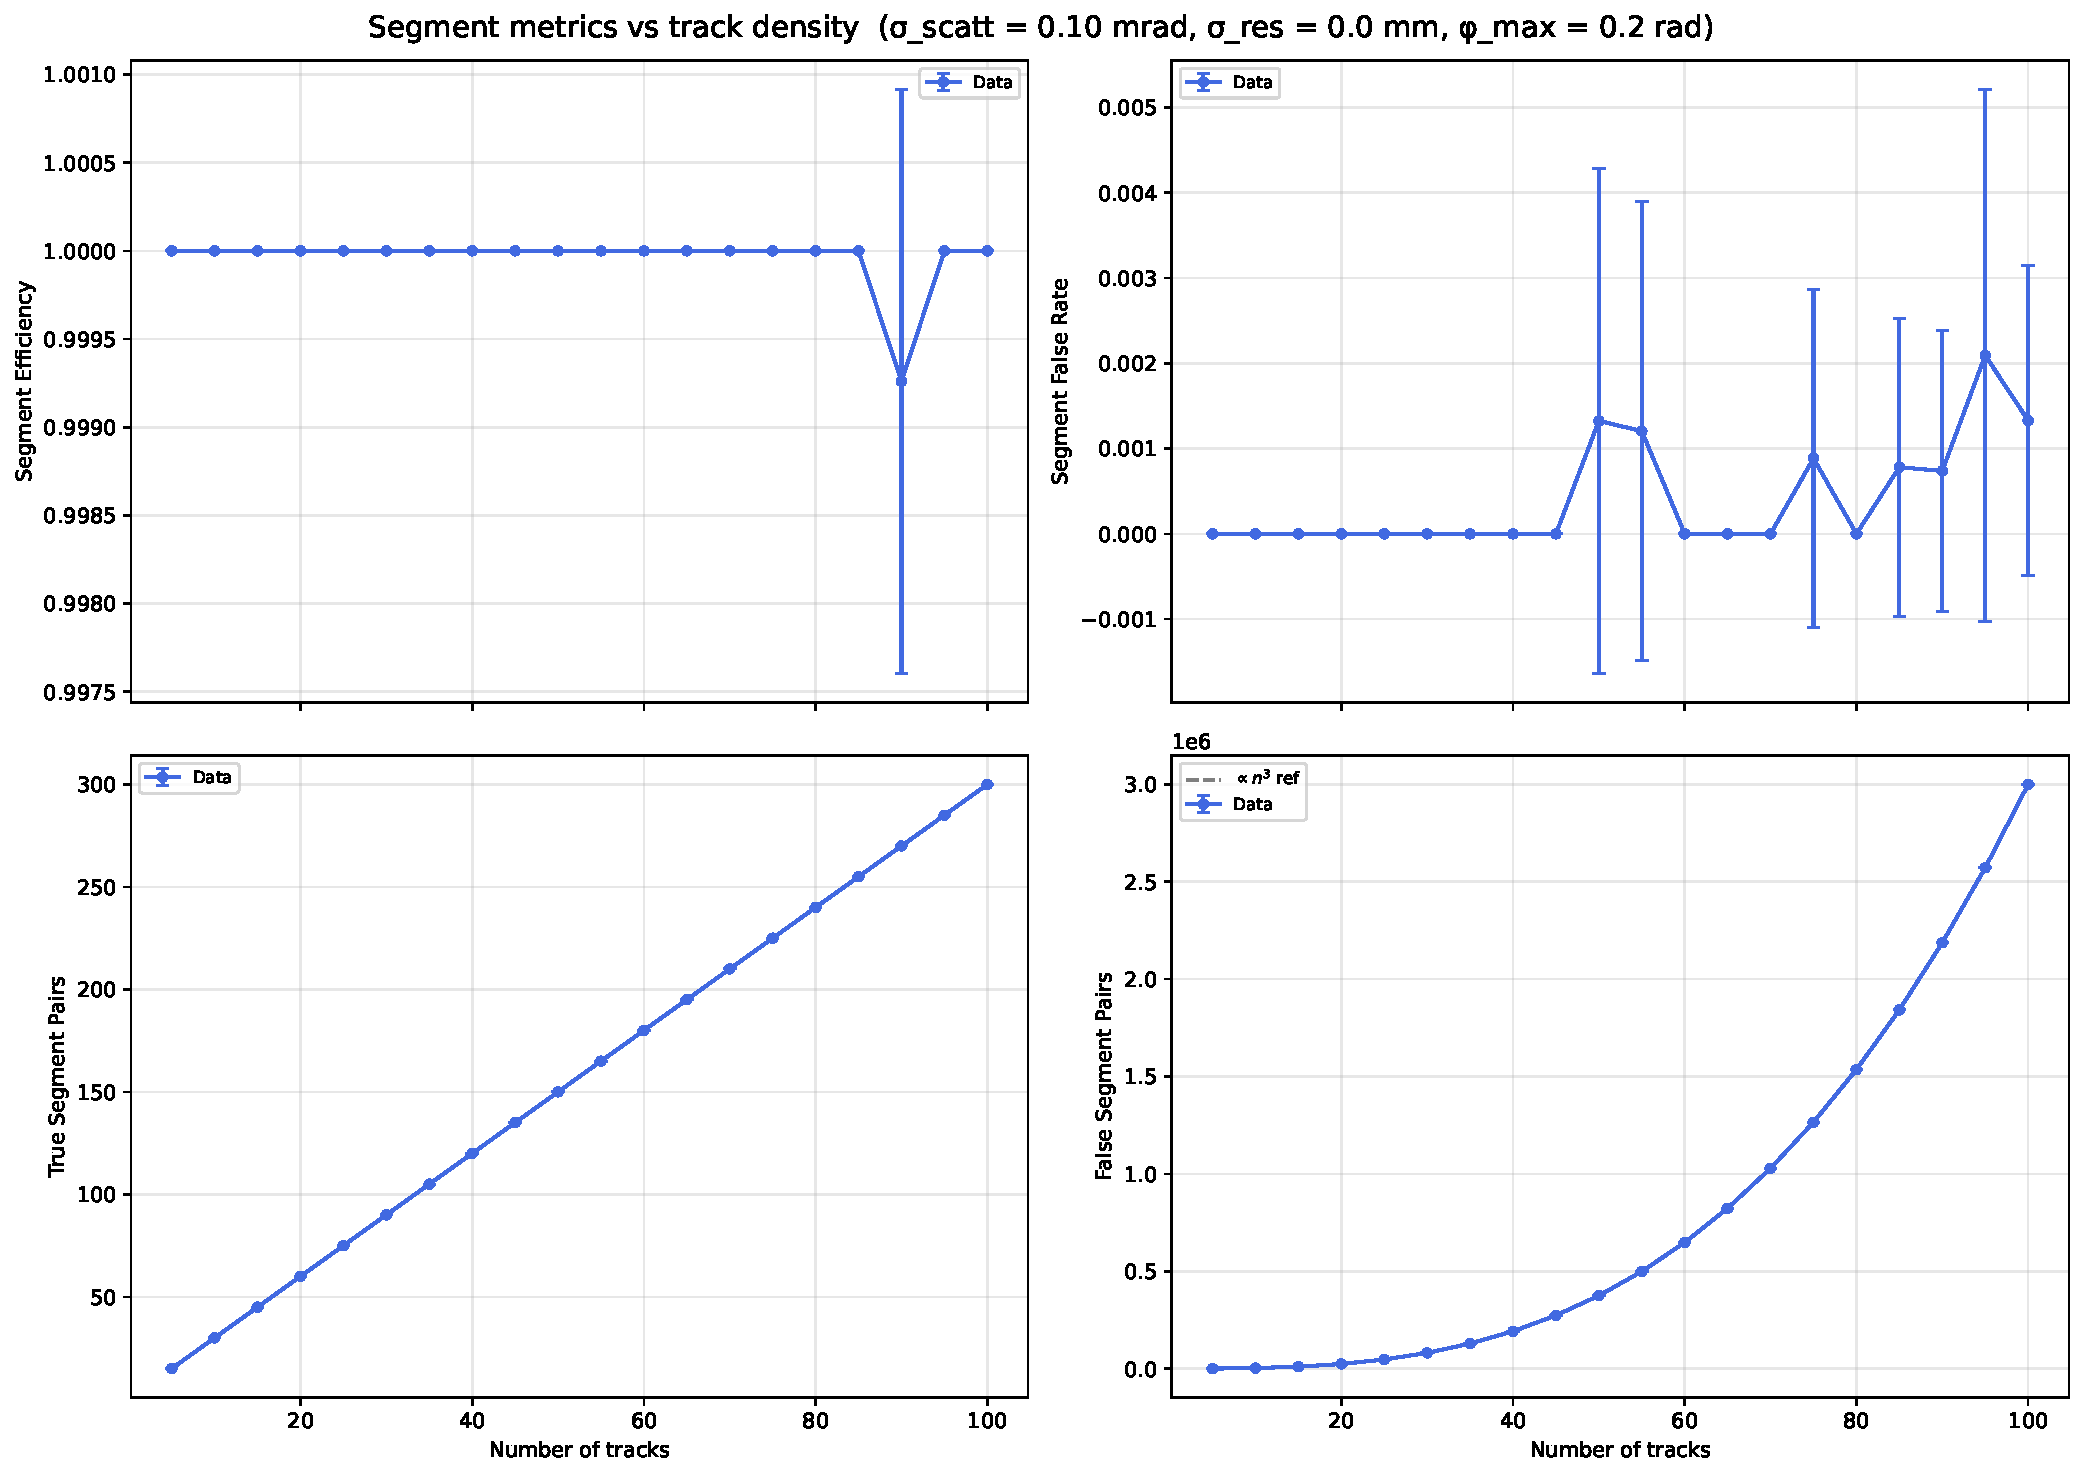
\includegraphics[width=0.7\linewidth]{density_scan.pdf}
  \caption{Density scan, $\nt = 5\dots100$, $\sss=0.1$~mrad, $\srr=0$.
  Panel (d) includes a reference $n^3$ slope.}
  \label{fig:density}
\end{figure}

\subsection{Fixed-$\eps$ comparison, new vs.\ old (\S10, \S10b, \S10c)}\label{sec:fixed-eps}
To reproduce the earlier reference notebook
\texttt{track\_density\_test\_local.ipynb}, the experiment is
re-run with identical generator parameters (MIP, PV
$\sigma=(1,1,1)$~mm, $160\times 160$~mm$^2$ modules,
$\sss=0.1$~mrad, $\srr=5\ \mu\mathrm{m}$) but under \emph{both}
segment-pair definitions of \S\ref{sec:method}, at a fixed
$\eps=2$~mrad. Segment efficiency is $100\%$ for both methods and at
every multiplicity. False rates diverge:
the triplet method produces a false pool growing as $T^3$, the
pairwise method as $T^2$. A weighted power-law fit $N = aT^b$ on the
false-pair counts recovers $b \approx 3$ (triplet) and $b \approx 2$
(pairwise), matching the combinatorial expectation
(Fig.~\ref{fig:newvsold}).

\begin{figure}[t]
  \centering
  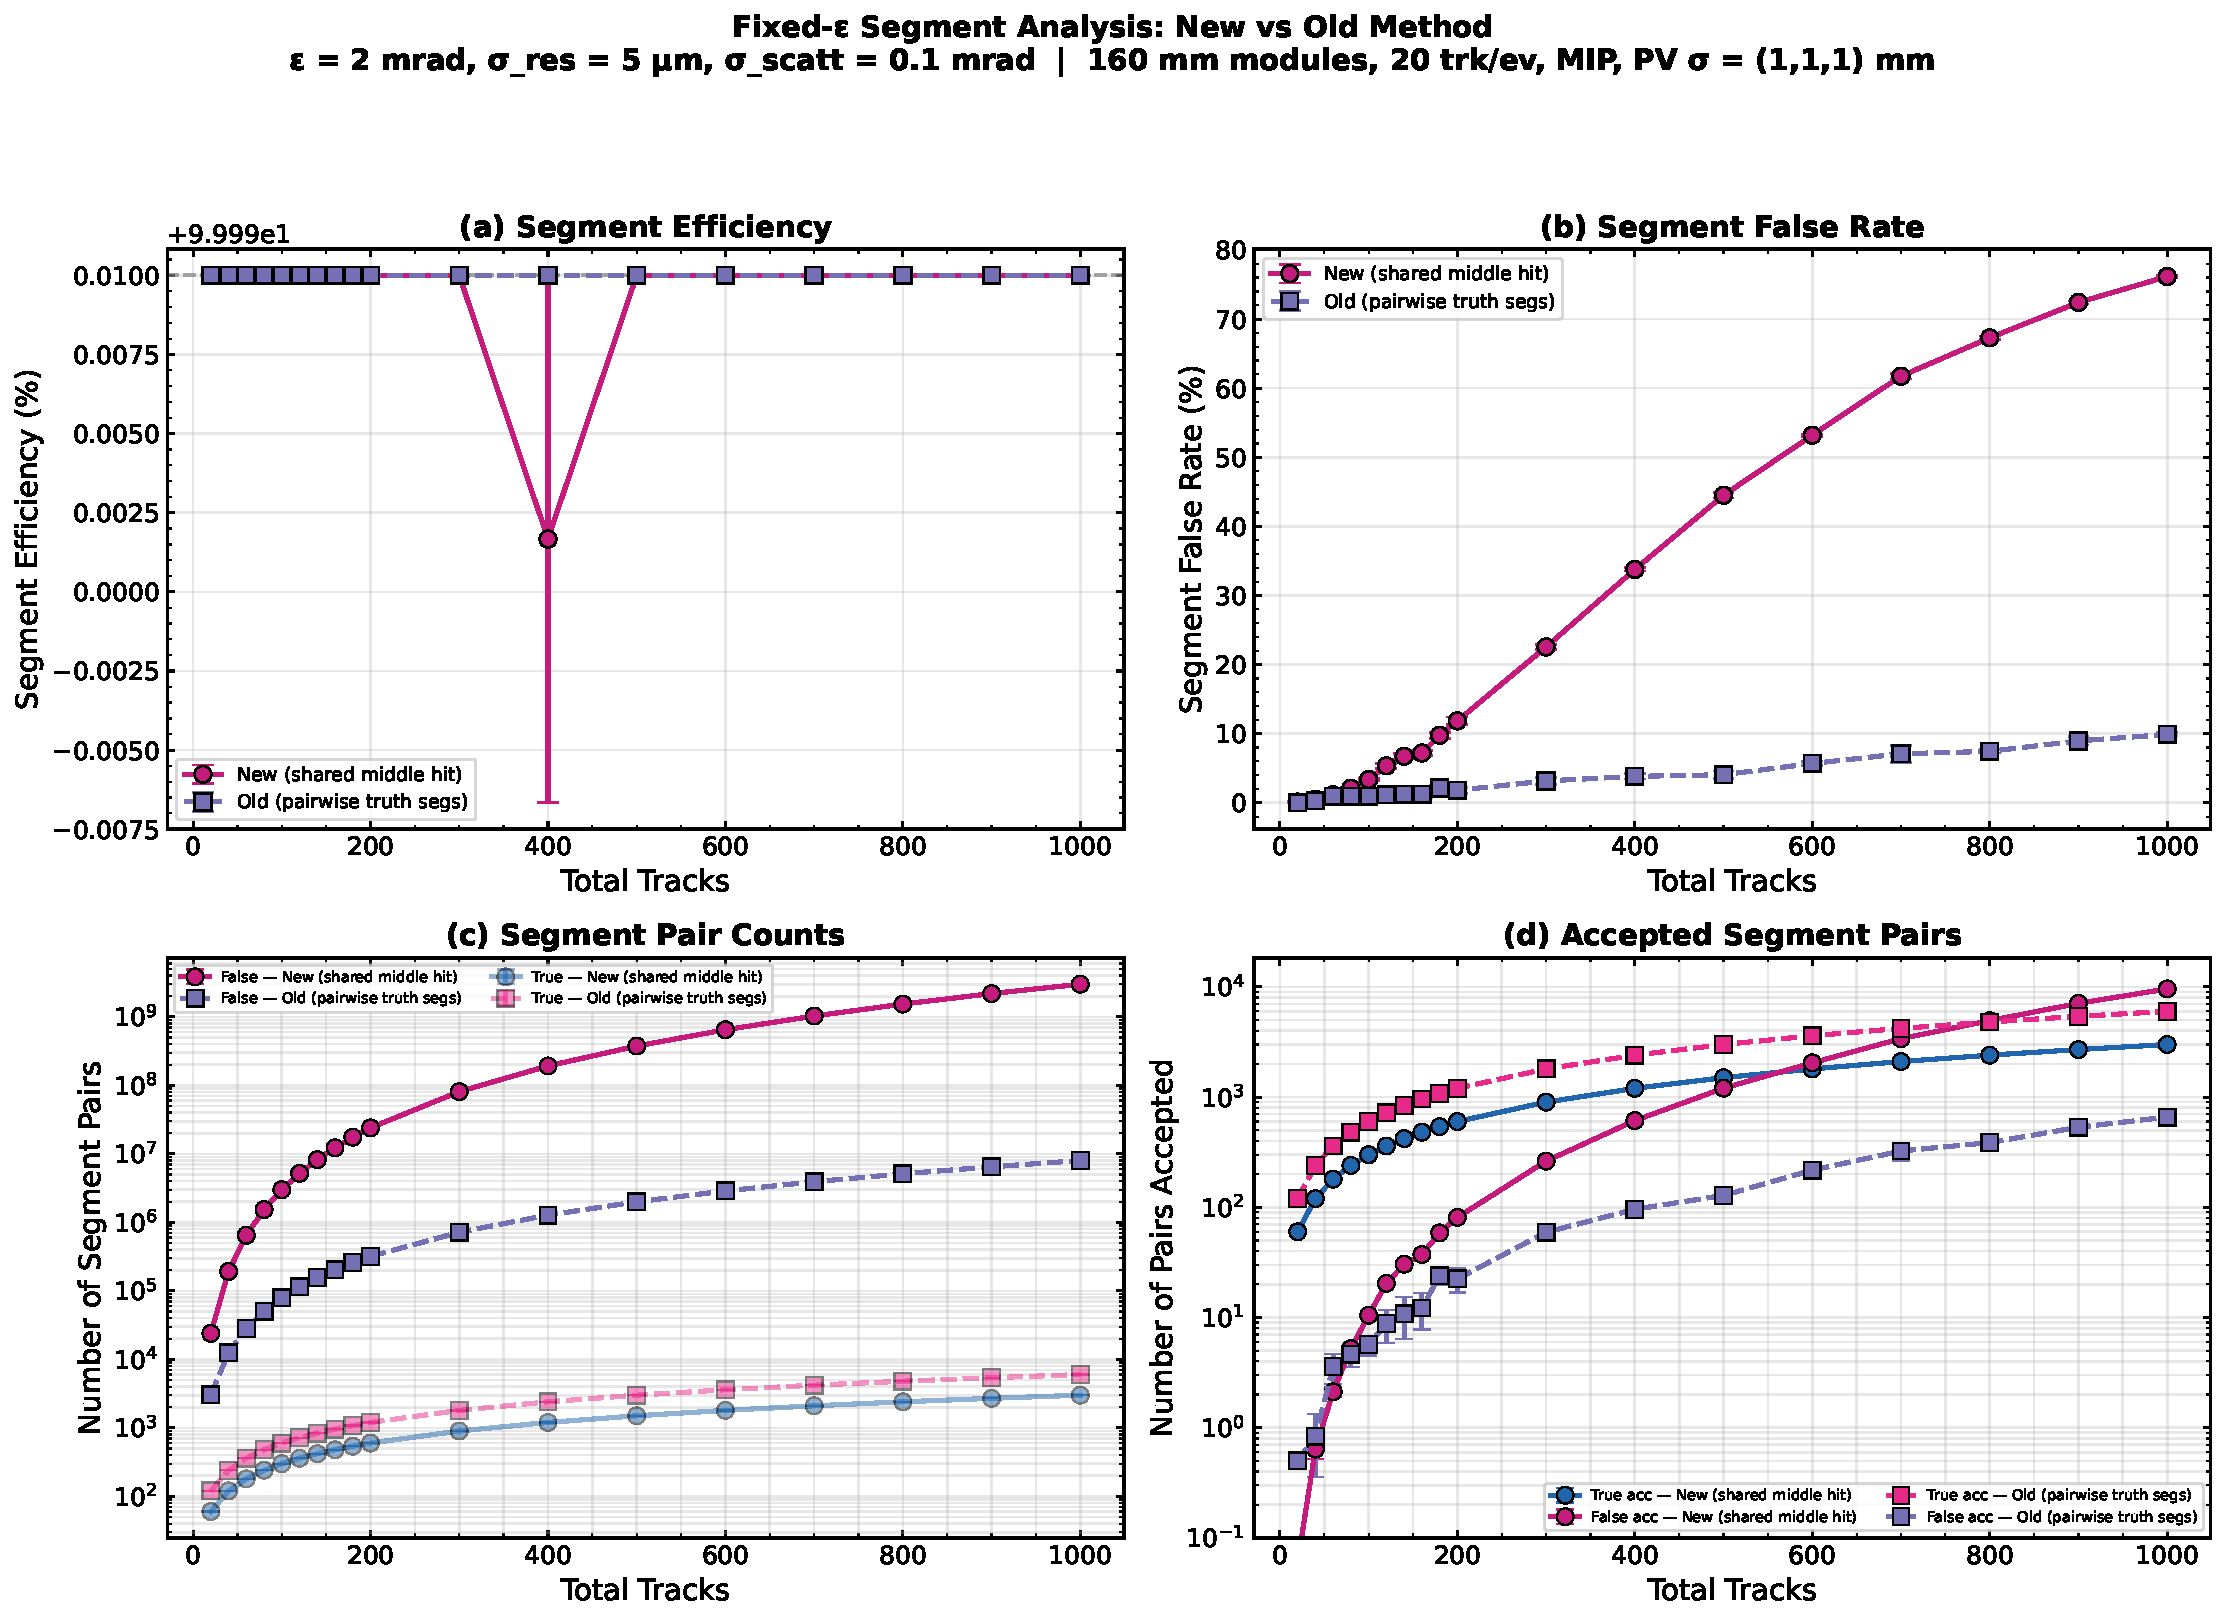
\includegraphics[width=0.48\linewidth]{fixed_epsilon_comparison_new_vs_old.pdf}\hfill
  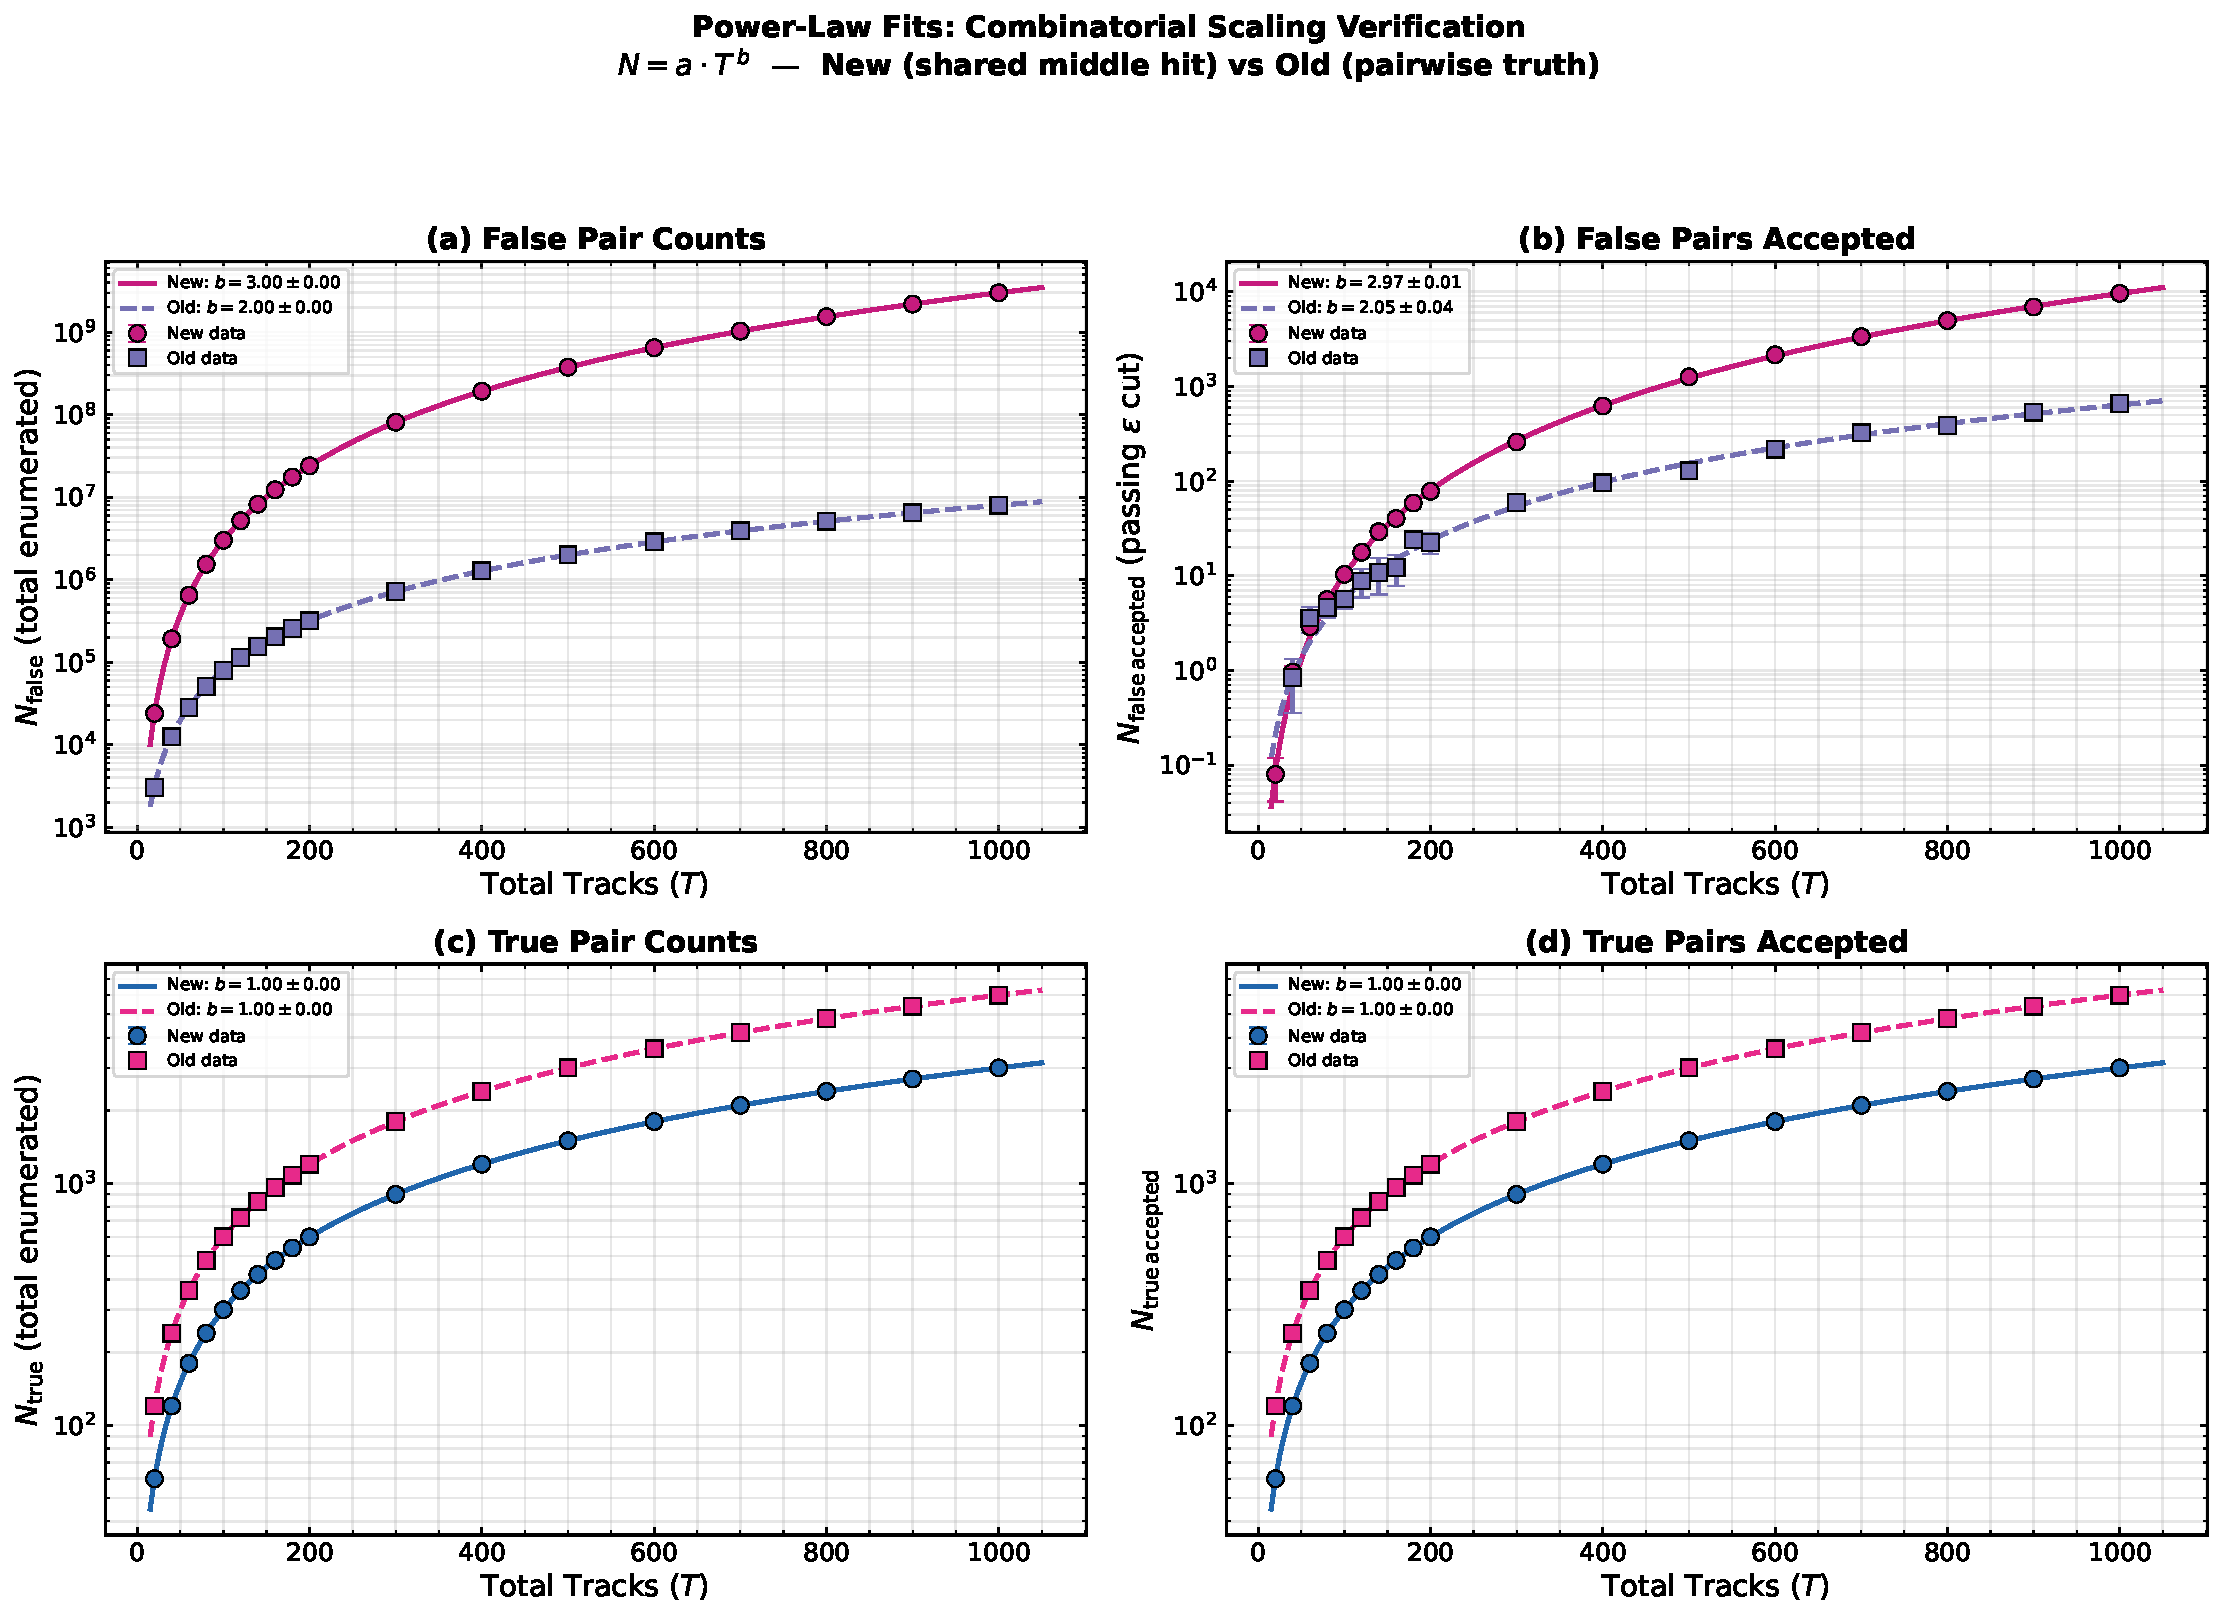
\includegraphics[width=0.48\linewidth]{scaling_power_law_fits_new_vs_old.pdf}
  \caption{Left: fixed-$\eps=2$~mrad efficiency/false-rate comparison
  between triplet (new) and pairwise (old-reference) metrics. Right:
  power-law fits of false- and true-pair counts vs.\ multiplicity,
  recovering the $b\approx 3$ (triplet) and $b\approx 2$ (pairwise)
  scalings. Source: \S10, \S10c.}
  \label{fig:newvsold}
\end{figure}

\subsection{Zero-noise benchmark (\S11)}
At $\sss \to 0$, $\srr=0$, $\eps$ collapses to the floor
$\sqrt{2}\,\theta_\mathrm{min} \approx 0.0212\ \mu\mathrm{rad}$.
Segment efficiency remains $\geq 95\%$ in both the dense
($\phi_\mathrm{max}=0.02$) and non-dense ($\phi_\mathrm{max}=0.2$)
regimes. The dense configuration shows a higher residual false-rate
floor due to coincidental alignment of small-angle tracks.

\subsection{Extended range to $10^3$ tracks (\S12, \S13)}\label{sec:extended}
Re-running \S5--\S7 and \S11 with $\nt$ extended to $\{200,500,1000\}$
(Numba-JIT triplet kernel) confirms all the scaling behaviours
observed at lower multiplicity. Segment efficiency stays at
$100\%$ at all tested combinations of $(\sss,\srr,\nt)$; false rate
tracks the combinatorial expectation. The paper-style 2$\times$2
figures for publication are in
\texttt{outputs/segment\_analysis/paper/fig13\{a--e\}.pdf}.

%--------------------------------------------------------------------
\section{Solver and track-level results}\label{sec:solver}

\subsection{Solver segment efficiency (\S14)}
Feeding the accepted triplets through the sparse Hopfield Hamiltonian
and thresholding at $\tau=0.35$ yields the four-panel
Fig.~\ref{fig:solver}: segment efficiency is flat at $100\%$ across
$\nt \in [2,1000]$. The false-rate (fraction of accepted segments
that are false) climbs from $0$ at low $\nt$ to $(19.8\pm 0.4)\%$
at $\nt=1000$. The raw pair counts in panel~(iii) again recover the
$n$ (true) and $n^3$ (false) slopes; the post-threshold counts in
panel~(iv) collapse the false count by several orders of magnitude
at low $\nt$ --- but at $\nt=1000$ the false-active count approaches
$10^3$ per event.

\begin{figure}[t]
  \centering
  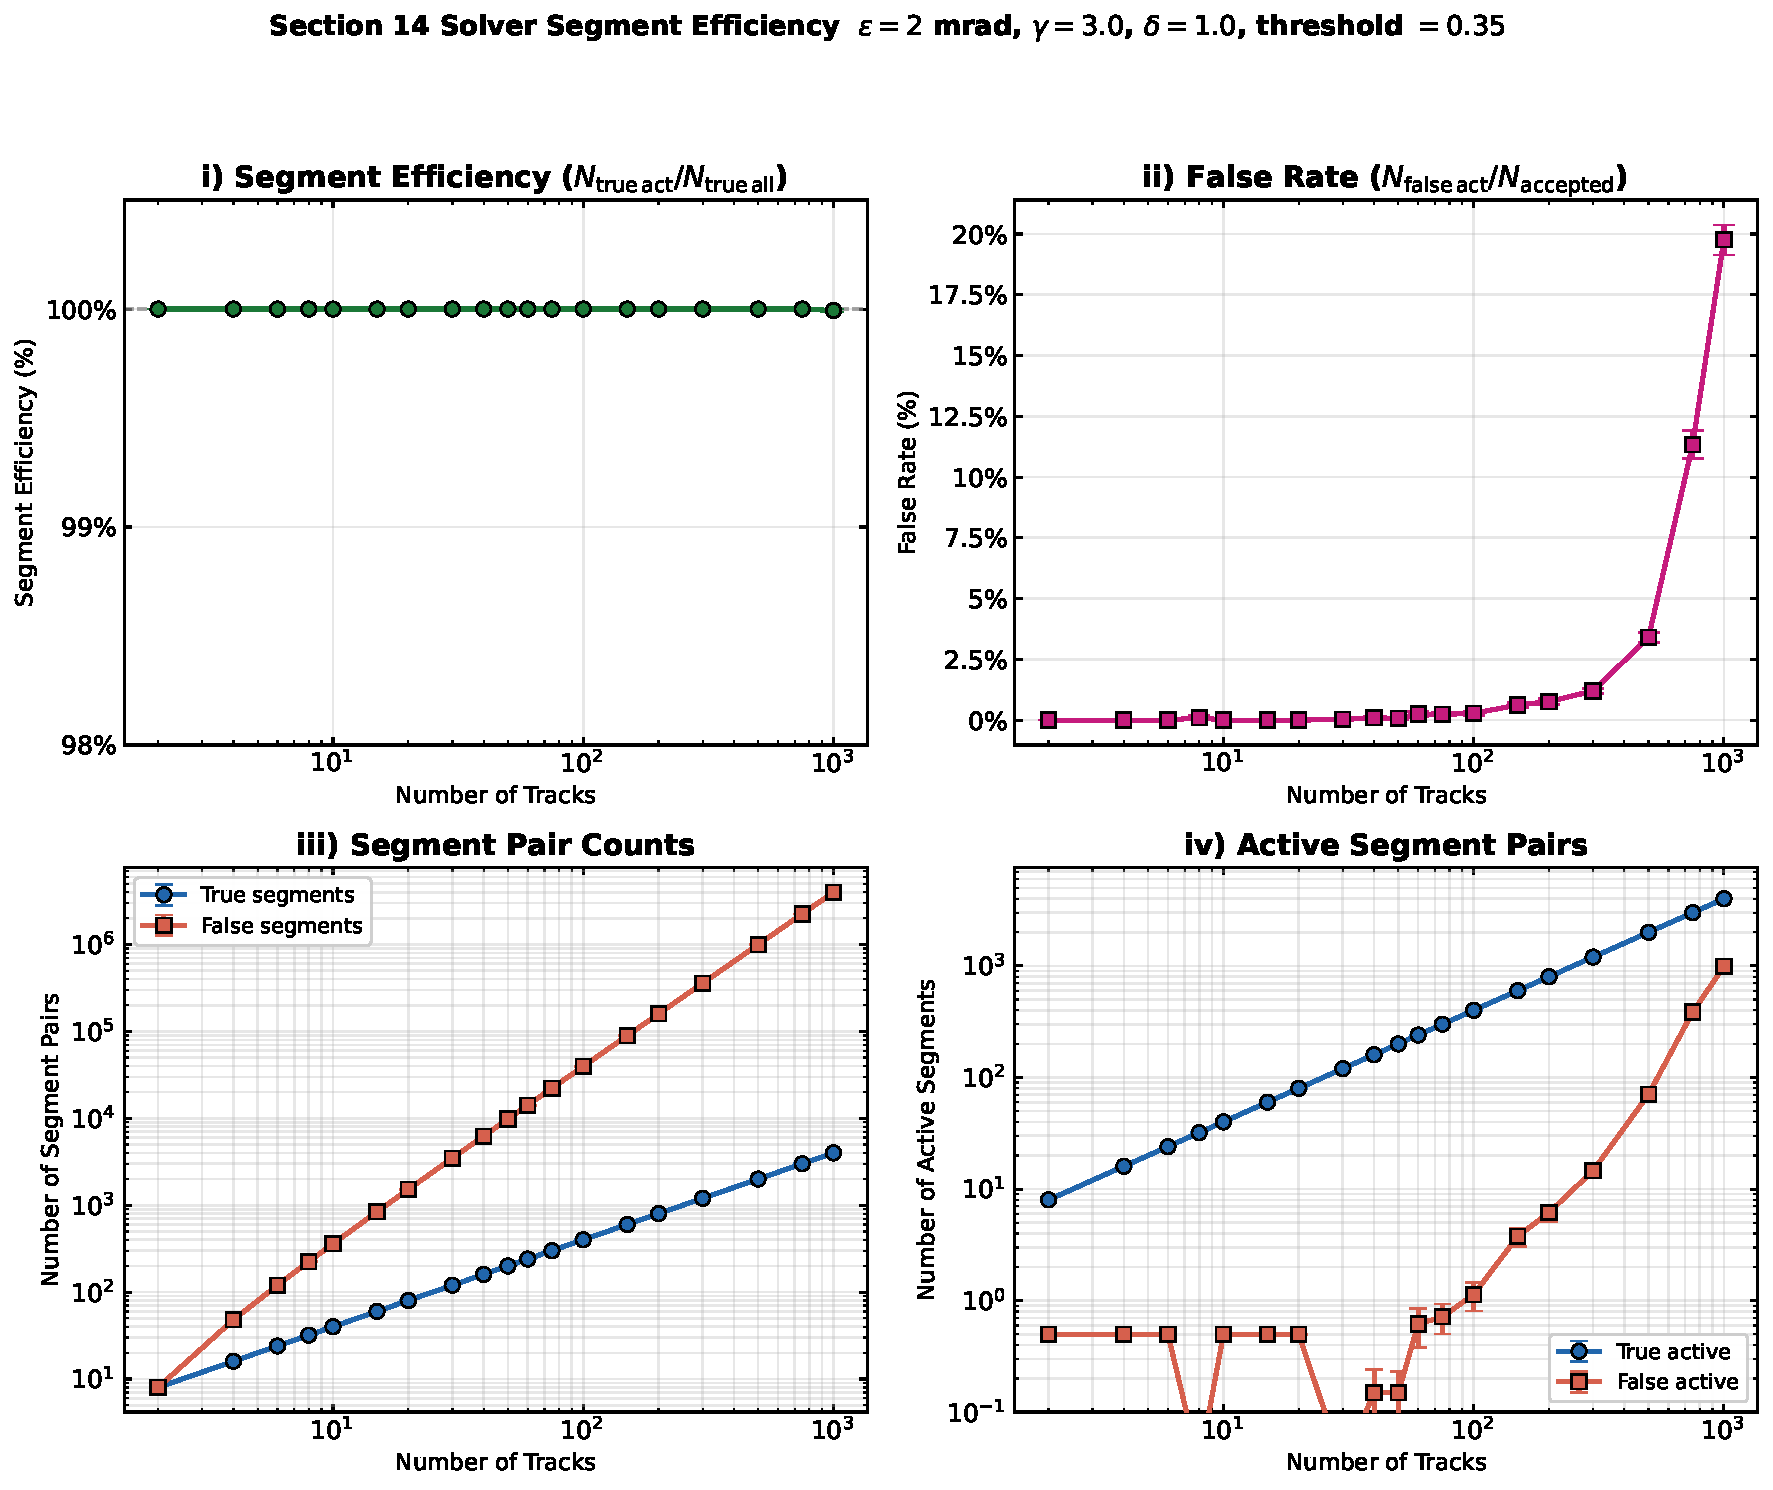
\includegraphics[width=0.9\linewidth]{paper/fig14_solver_segment_efficiency_logx.pdf}
  \caption{\S14: Solver segment efficiency (i), false rate (ii),
  raw pair counts (iii), and post-threshold active counts (iv)
  versus multiplicity. $\gamma=3$, $\delta=1$, $\eps=2$~mrad,
  $\tau=0.35$.}
  \label{fig:solver}
\end{figure}

\subsection{Track-level performance and the knee (\S15)}
Figure~\ref{fig:tracks} shows the six-panel track-level summary
from \texttt{EventValidator}. Reconstruction efficiency plateaus
at $\approx 99\%$ up to $\nt=500$, drops to $\approx 85\%$ at
$\nt=750$, and collapses to $(44\pm 3)\%$ at $\nt=1000$. The ghost
rate peaks at $\approx 3.3\%$ near $\nt=500$--$750$ then
\emph{falls} at $\nt=1000$ --- not because ghosts vanish, but because
the connected-component tracker absorbs false-segment bridges into
mega-clusters which fail the purity cut and therefore neither count
as matched nor as ghost-reco. Clone fraction is numerically zero.
Mean purity of accepted tracks remains $=1.00$; mean hit efficiency
is $1.000$ for clean events and $(0.996\pm 0.002)$ under a $1\%$
hit-drop model, consistent with the structural loss expected from
dropping on average one hit per five.

\begin{figure}[t]
  \centering
  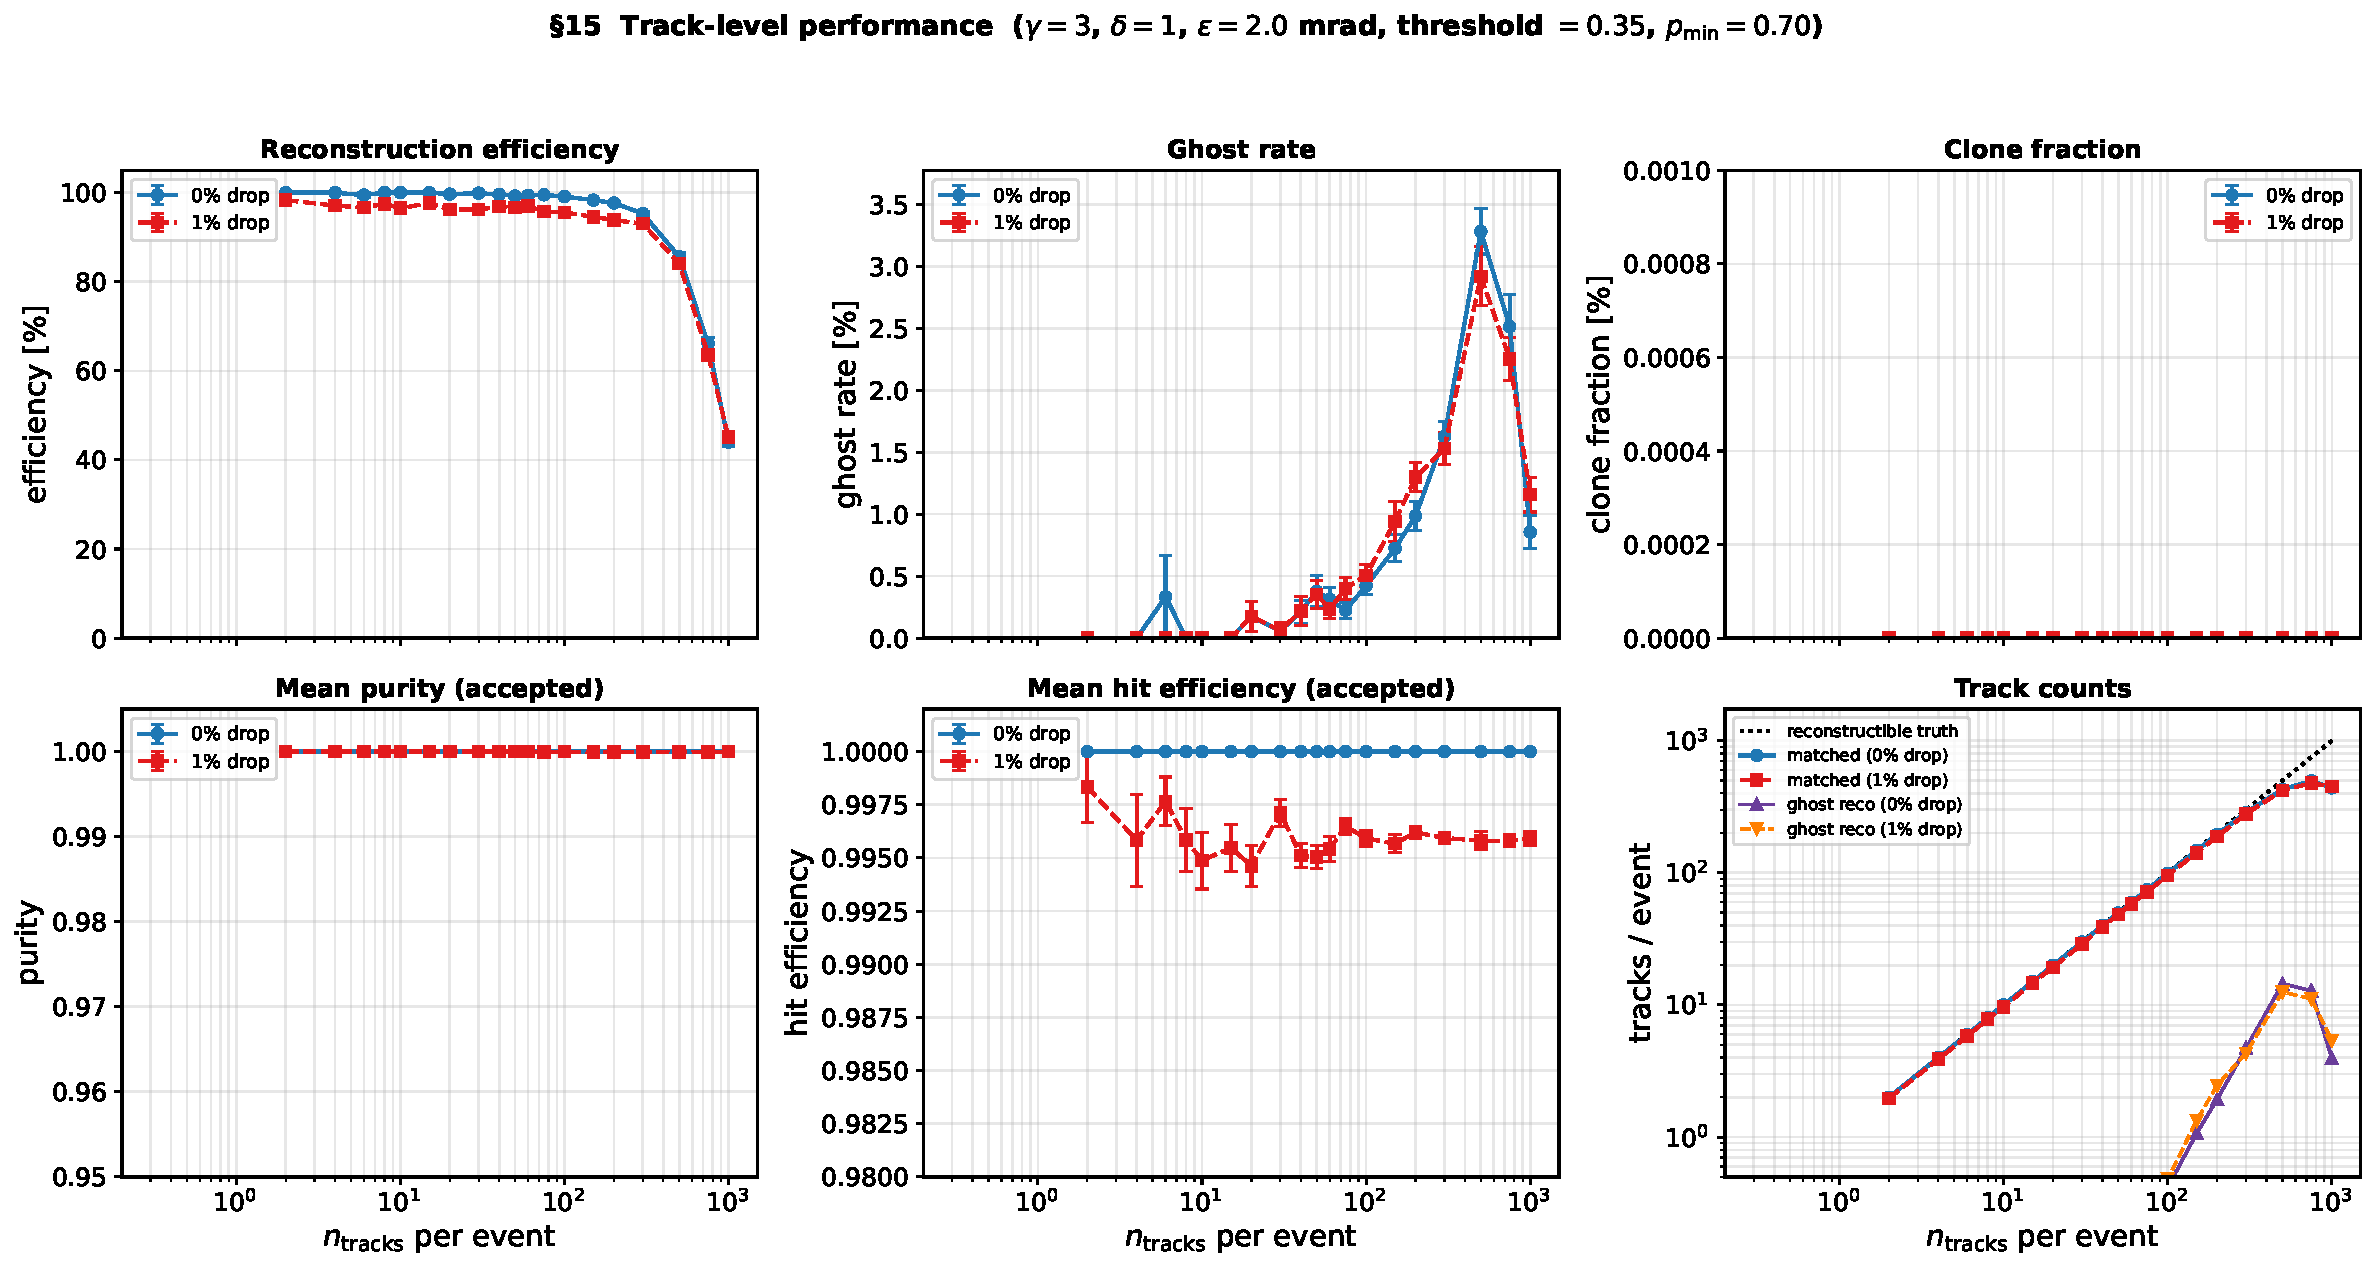
\includegraphics[width=\linewidth]{fig15_track_level_overlay.pdf}
  \caption{\S15: track-level metrics under
  \texttt{EventValidator.match\_tracks} with purity $\geq 0.70$,
  \texttt{min\_rec\_hits}$=3$, for clean and $1\%$ hit-drop events.
  The efficiency knee appears between $\nt = 500$ and $\nt = 1000$.}
  \label{fig:tracks}
\end{figure}

\subsection{Spectral diagnostics (\S16)}
To determine whether the efficiency collapse originates in the
solver, the Hamiltonian matrix is analysed by sparse ARPACK
eigensolve \cite{Lehoucq:1998:arpack}. The results are summarised in
Table~\ref{tab:spec} and Fig.~\ref{fig:spec}. The minimum eigenvalue
bottoms out at $\lambda_\mathrm{min}=0.88$ for $\nt\geq 750$; the
maximum eigenvalue saturates at $\lambda_\mathrm{max}\approx 7.1$; the
condition number remains bounded by $\kappa \lesssim 9$. The
Gershgorin lower bound $\min_i(d_i-r_i)$ saturates at zero for
$\nt \geq 500$, indicating that the coupling mass per row matches
the diagonal, but ARPACK confirms the actual spectrum stays strictly
positive: the matrix is everywhere invertible and the SPD direct
solve is numerically healthy.

\begin{table}[t]
  \caption{Spectral quantities of the Hopfield Hamiltonian at fixed
  $(\gamma,\delta,\eps)=(3,1,2\,\mathrm{mrad})$.
  \label{tab:spec}}
  \centering
  \begin{tabular}{rcccc}
    \toprule
    $\nt$ & $\lambda_\mathrm{min}$ & $\lambda_\mathrm{max}$ & $\kappa$ & $\max_i r_i$ \\
    \midrule
    10    & 2.38 & 5.62 & 2.36 & 2.0 \\
    100   & 2.22 & 5.80 & 2.61 & 2.7 \\
    300   & 1.98 & 6.00 & 3.03 & 3.0 \\
    500   & 1.02 & 6.94 & 7.5  & 4.0 \\
    750   & 0.88 & 7.12 & 8.6  & 4.0 \\
    1000  & 0.88 & 7.12 & 8.2  & 4.0 \\
    \bottomrule
  \end{tabular}
\end{table}

\begin{figure}[t]
  \centering
  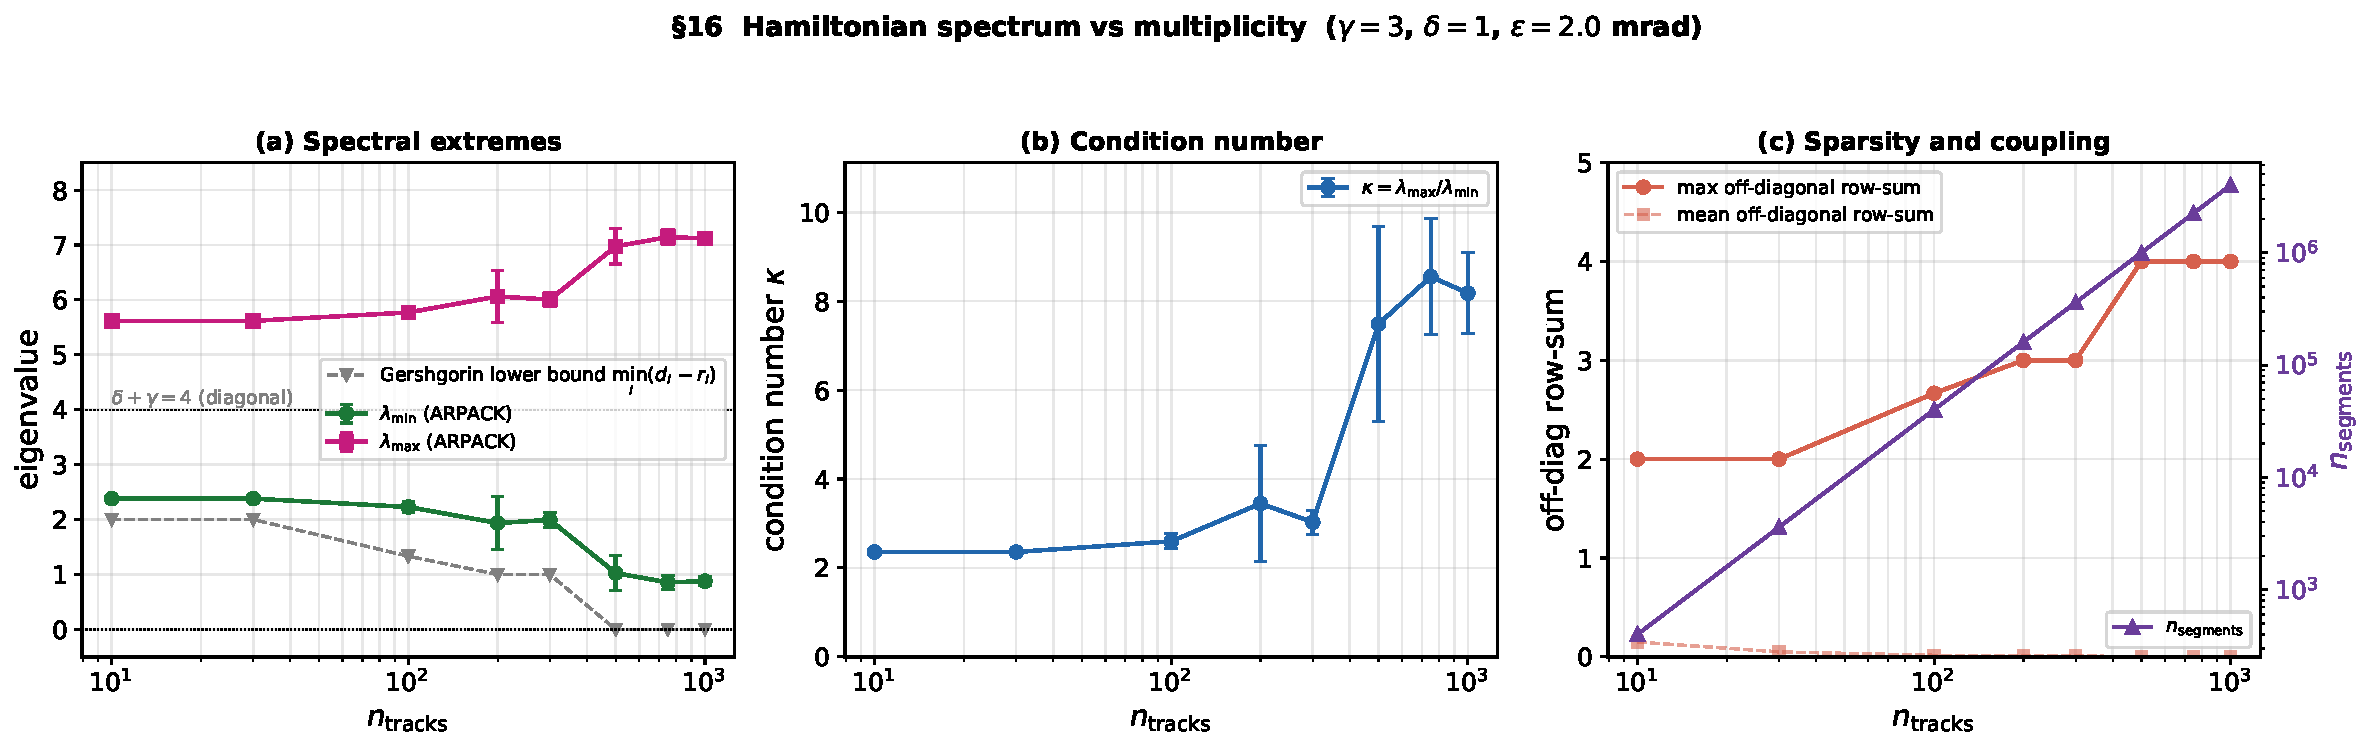
\includegraphics[width=\linewidth]{fig16_spectrum.pdf}
  \caption{\S16: extremal eigenvalues, condition number, and
  off-diagonal row-sum versus multiplicity.}
  \label{fig:spec}
\end{figure}

\subsection{Solution histograms (\S16c)}
The per-segment solution distribution (Fig.~\ref{fig:hist}) shows a
tight false-segment peak at the isolated-Hopfield fixed point
$s^\ast_\mathrm{fp}=\delta/(\delta+\gamma)=0.25$ and a broader true-segment
population with outer-chain invariant $s^\ast_\mathrm{outer}=0.3636$. At
all tested multiplicities the threshold $\tau=0.35$ separates the
peaks cleanly. A small high-$s$ false-tail emerges at large $\nt$
(Table~\ref{tab:fp}): $0$, $9$, $32$, $306$, $1119$, $2788$ false
activations at $\nt\in\{10,100,300,500,750,1000\}$, translating to a
false-rate of $0.00\%$--$0.02\%$ of the total false pool --- which is
nonetheless a large \emph{absolute} number at high multiplicity
because the false pool itself scales as $\nt^3$.

\begin{figure}[t]
  \centering
  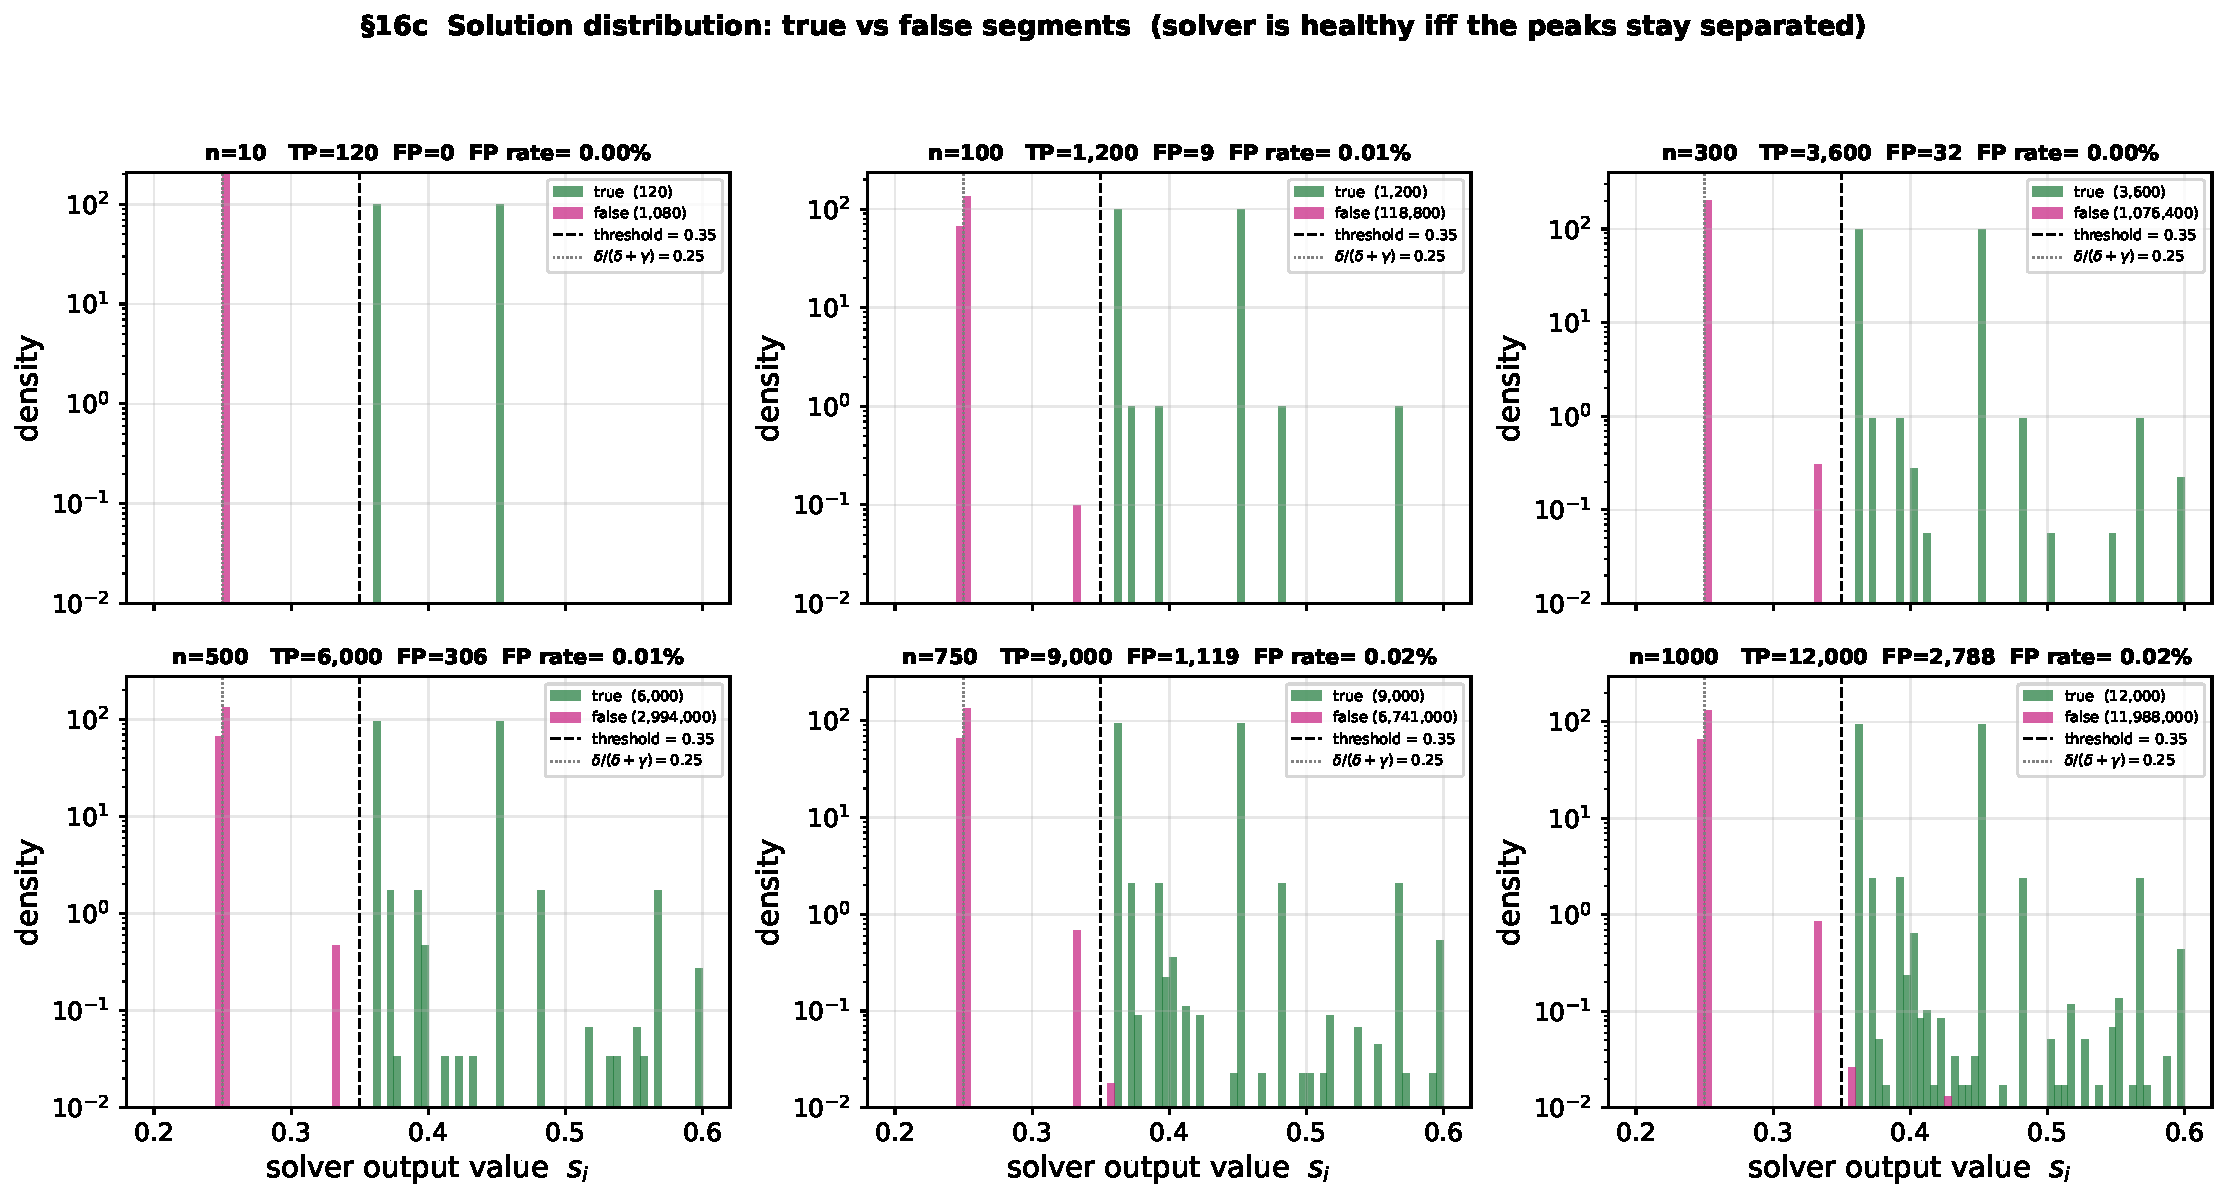
\includegraphics[width=\linewidth]{fig16c_solution_histograms.pdf}
  \caption{\S16c: solver output distributions for true (green) and
  false (magenta) segments. Dashed: threshold $\tau=0.35$; dotted:
  $s^\ast_\mathrm{fp}=0.25$.}
  \label{fig:hist}
\end{figure}

\begin{table}[t]
  \centering
  \caption{False-positive counts from \S16c.\label{tab:fp}}
  \begin{tabular}{rrrr}
    \toprule
    $\nt$ & TP & FP $>\tau$ & FP fraction \\
    \midrule
    10   & 120    & 0    & 0.00\% \\
    100  & 1\,200  & 9    & 0.01\% \\
    300  & 3\,600  & 32   & 0.00\% \\
    500  & 6\,000  & 306  & 0.01\% \\
    750  & 9\,000  & 1\,119 & 0.02\% \\
    1000 & 12\,000 & 2\,788 & 0.02\% \\
    \bottomrule
  \end{tabular}
\end{table}

\subsection{Tracker A/B (\S17)}\label{sec:ab}
The same set of solver-active segments is fed into two trackers
(Table~\ref{tab:ab}, Fig.~\ref{fig:ab}). The connected-component
tracker (\texttt{get\_tracks}) and the layered tracker
(\texttt{get\_tracks\_layered}) share the same solver output but
differ dramatically in their high-$\nt$ behaviour: CC efficiency
collapses from $98.8\%$ at $\nt=100$ to $42.8\%$ at $\nt=1000$,
whereas the layered tracker remains at $\geq 99.96\%$ across the same
range. The layered tracker pays with a ghost rate that grows from
$0.1\%$ to $23.6\%$ over the same span, produced almost entirely by
the small-but-rising high-$s$ false tail of
\S\ref{sec:solver}.

\begin{table}[t]
  \centering
  \caption{\S17: tracker A/B comparison (clean events).\label{tab:ab}}
  \begin{tabular}{rcccc}
    \toprule
    $\nt$ & eff (CC) & eff (layered) & ghost (CC) & ghost (layered) \\
    \midrule
    100  & 98.8\% & 100.0\% & 0.5\% & 0.1\% \\
    300  & 94.7\% & 100.0\% & 0.9\% & 1.2\% \\
    500  & 85.4\% & 100.0\% & 1.6\% & 3.9\% \\
    750  & 67.1\% & 99.96\% & 3.3\% & 11.7\% \\
    1000 & 42.8\% & 99.98\% & 0.9\% & 23.6\% \\
    \bottomrule
  \end{tabular}
\end{table}

\begin{figure}[t]
  \centering
  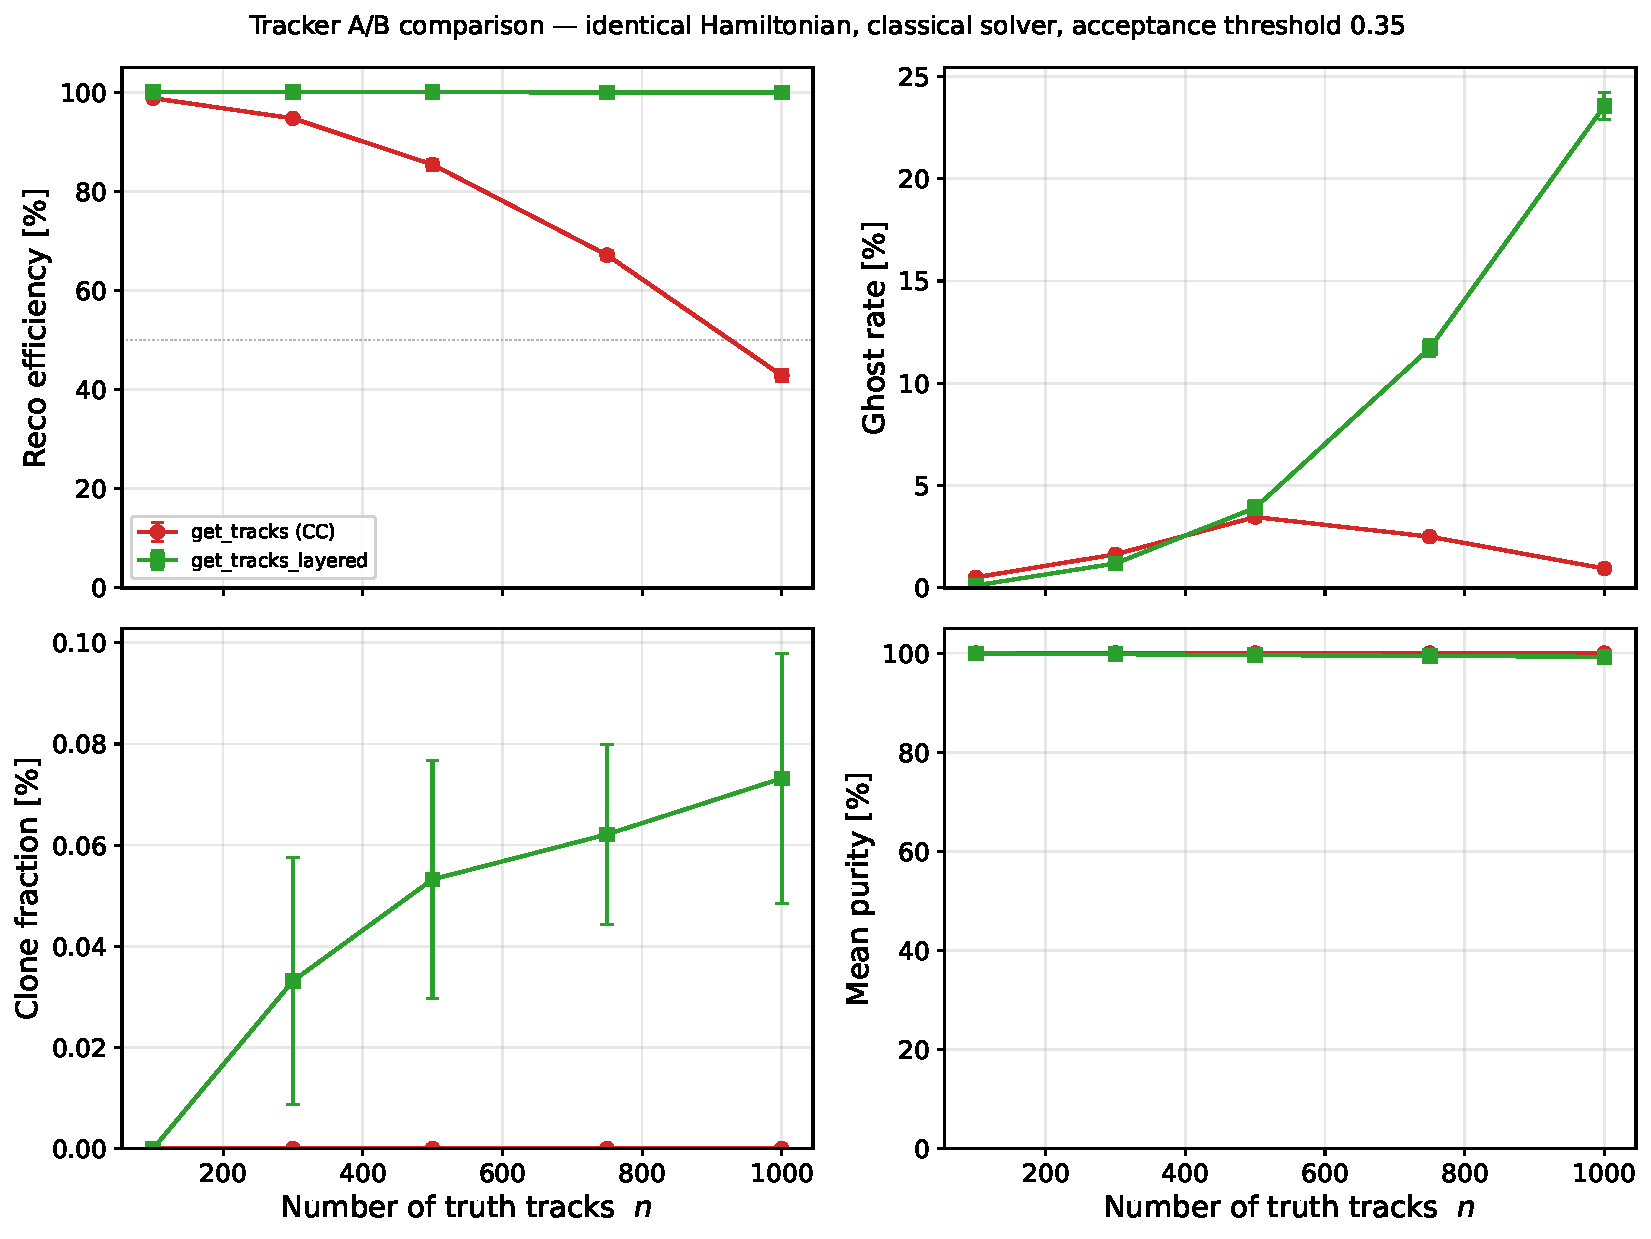
\includegraphics[width=0.9\linewidth]{fig17_tracker_ab.pdf}
  \caption{\S17: reconstruction efficiency and ghost rate for the two
  trackers, same solver output.}
  \label{fig:ab}
\end{figure}

%--------------------------------------------------------------------
\section{Discussion}\label{sec:discussion}

The results in \S\ref{sec:segment} demonstrate that the analytic
threshold $\eps(\sss,\srr)$ is \emph{overtight} only by the safety
factor $s=3$ it was constructed with: true-pair acceptance stays at
$100\%$ across the full sweep grid and the observed false-rate climb
is entirely due to the combinatorial growth of the false-pair pool,
not to a mismatched $\eps$. The triplet/pairwise comparison in
\S\ref{sec:fixed-eps} recovers exactly the expected $T^3$ and $T^2$
combinatorial scalings, and so the new package reproduces the older
reference to within statistical error --- the only genuine difference
between them is the choice of segment-pair definition.

The high-multiplicity behaviour identified in \S\ref{sec:solver}
is the central finding of this study. The solver itself remains
healthy: the Hamiltonian spectrum is strictly positive, the matrix
is sparse and well-conditioned ($\kappa \leq 9$), and the per-segment
solution populations show the expected Hopfield fixed points
$s^\ast_\mathrm{fp}=0.25$ and $s^\ast_\mathrm{outer}=0.3636$
with threshold-preserving separation at all tested $\nt$. The
false-rate growth at high $\nt$ is therefore structural, not
numerical: with $\mathcal{O}(\nt^3)$ false-pair candidates, even an
$\mathcal{O}(10^{-4})$ post-threshold misclassification rate produces
$\mathcal{O}(10^3)$ ghost segments per event at $\nt=1000$.

The resulting tracker failure (Fig.~\ref{fig:ab}) is a post-processing
artefact: the connected-component algorithm treats the false-segment
"bridges" as legitimate edges and merges entire bundles of real tracks
into unmatchable super-clusters; the layered tracker, by contrast,
imposes module-exclusivity and angular consistency, rejects
bridging segments, and recovers $\geq 99.9\%$ reconstruction
efficiency --- at the price of a $23.6\%$ ghost rate at $\nt=1000$.
The validated Hamiltonian operating point $(\gamma,\delta,\eps,\tau) =
(3,\,1,\,2\,\mathrm{mrad},\,0.35)$ therefore supports up to $\nt =
10^3$ tracks per event with either tracker, at opposite ends of the
efficiency-vs-purity trade-off.

\paragraph{Limitations.}
\begin{itemize}
  \item The spectrum scan (\S16) uses a single event per multiplicity
        point; the error bars on $\lambda_\mathrm{max}$ at high $\nt$
        are indicative only.
  \item Only a $1\%$ flat hit-drop model is tested; no ghost-hit or
        module-inefficiency models are included.
  \item The $s\approx 0.45$--$0.6$ false-tail at $\nt=1000$
        (Fig.~\ref{fig:hist}) is not characterised in detail;
        tightening $\tau$ or raising $\gamma$ would suppress it at
        some cost to the true-peak lower tail.
\end{itemize}

%--------------------------------------------------------------------
\section{Conclusion}\label{sec:conclusion}

The \texttt{lhcb\_velo\_toy} stack has been verified against the
earlier reference implementation and characterised up to
$\nt = 10^3$ tracks per event. Within the validated envelope
$(\gamma,\delta,\eps,\tau) = (3,\,1,\,2\,\mathrm{mrad},\,0.35)$, the
Hamiltonian segment solver is numerically healthy and delivers
$100\%$ segment efficiency. The efficiency collapse observed with the
default connected-components tracker is a \emph{tracker} artefact and
is fully reversed by a module-exclusive layered tracker.

%--------------------------------------------------------------------
\bibliographystyle{unsrtnat}
\bibliography{refs}

%--------------------------------------------------------------------
% TODO outstanding:
%  * Extract exact fitted exponents from \S10c (cell #VSC-ae61d74f) if
%    quantitative scaling is needed in the abstract.
%  * Replace the \cite{Nilles:2023:qtracking} placeholder with the
%    actual OBQF paper reference once located.
%  * Add 1% drop column to Tab.~\ref{tab:ab} if desired.
%  * Consider a supplementary appendix showing the full \S10c
%    power-law fit table.
%  * Quantify the high-$s$ false tail at \nt=1000 (Fig.~\ref{fig:hist})
%    with a gamma- or threshold-sensitivity sub-study.

\end{document}
